% arara: xelatex
% arara: xelatex
% arara: xelatex

% options:
% thesis=B bachelor's thesis
% thesis=M master's thesis
% czech thesis in Czech language
% english thesis in English language
% hidelinks remove colour boxes around hyperlinks

\documentclass[thesis=M,czech]{FITthesis}[2018/10/20]

\usepackage[utf8]{inputenc} % LaTeX source encoded as UTF-8
\usepackage{graphicx} %graphics files inclusion
\usepackage{listings}
\usepackage{pgfplots}
\usepackage[czech]{babel}
\usepackage{lmodern} 
\usepackage[T1]{fontenc}
\usepackage{float}
\usepackage{subfig}
\usepackage{multirow}
% \usepackage{subfig} %subfigures
% \usepackage{amsmath} %advanced maths
% \usepackage{amssymb} %additional math symbols
\usepackage[acronym,nonumberlist,toc,numberedsection=autolabel]{glossaries}
\usepackage{dirtree} %directory tree visualisation

% list of acronyms
% \usepackage[acronym,nonumberlist,toc,numberedsection=autolabel,nomain]{glossaries}
\iflanguage{czech}{\renewcommand*{\acronymname}{Seznam použitých zkratek}}{}
% \makeglossaries

% % % % % % % % % % % % % % % % % % % % % % % % % % % % % % % % % % % 
% % % % % % % % % % % % % % % % % % % % % % % % % % % % % % % % % % % 
\department{Katedra softwarového inženýrství}
\title{Webové prostředí pro správu a konfiguraci IoT projektů}
\authorGN{Jakub} %author's given name/names
\authorFN{Vejr} %author's surname
\authorWithDegrees{Bc. Jakub Vejr} %author's name with academic degrees
\author{Jakub Vejr} %author's name without academic degrees
\supervisor{Ing. Stanislav Vítek, Ph.D.}
\acknowledgements{Rád bych poděkoval Ing. Stanislavu Vítkovi, Ph.D za vedení práce a všem lidem, kteří mne při vypracování této práce podporovali.}
\abstractCS{
Diplomová práce se zabývá návrhem a implementací webové aplikace pro správu a konfiguraci IoT projektů. Její dílčí cíle jsou umožnit, aby aplikace mohla shromažďovat data z IoT senzorů, ukládat tato data a následně je prezentovat uživatelům aplikace. Řešení bylo naprogramováno v jazyku JavaScript za použití frameworků Next.js a Express.
}
\website{https://github.com/vejrak/jv-dp}

\abstractEN{
The goal of this master thesis is to design and implement a web application for managing and configuration IoT projects.  The partial goal is to enable collecting and saving data from IoT sensors and present these data to the application users. The result was developed in JavaScript language using Next.js and Express frameworks.
}
\placeForDeclarationOfAuthenticity{Prague} %where you have signed the declaration
\keywordsCS{IoT, shromažďování dat, webová aplikace, Node.js, Next.js
\newpage}
\keywordsEN{IoT, data collecting, web application, Node.js, Next.js}
\declarationOfAuthenticityOption{4} %select as appropriate, according to the desired license
%\website{http://site.example/thesis} %optional URL (remove entirely if you have no URL for this thesis)
\usepackage{courier}

\lstset{basicstyle=\footnotesize\ttfamily,breaklines=true}
\lstset{
    inputencoding=utf8,
    extendedchars=true,
    literate=%
    {á}{{\'a}}1
    {č}{{\v{c}}}1
    {ď}{{\v{d}}}1
    {é}{{\'e}}1
    {ě}{{\v{e}}}1
    {í}{{\'i}}1
    {ň}{{\v{n}}}1
    {ó}{{\'o}}1
    {ř}{{\v{r}}}1
    {š}{{\v{s}}}1
    {ť}{{\v{t}}}1
    {ú}{{\'u}}1
    {ů}{{\r{u}}}1
    {ý}{{\'y}}1
    {ž}{{\v{z}}}1
    {Á}{{\'A}}1
    {Č}{{\v{C}}}1
    {Ď}{{\v{D}}}1
    {É}{{\'E}}1
    {Ě}{{\v{E}}}1
    {Í}{{\'I}}1
    {Ň}{{\v{N}}}1
    {Ó}{{\'O}}1
    {Ř}{{\v{R}}}1
    {Š}{{\v{S}}}1
    {Ť}{{\v{T}}}1
    {Ú}{{\'U}}1
    {Ů}{{\r{U}}}1
    {Ý}{{\'Y}}1
    {Ž}{{\v{Z}}}1
}
\begin{document}
% \newacronym{LZW}{LZW}{Lempel Ziv Welch}
% \newacronym{RLE}{RLE}{Run-Length Encoding}

\begin{introduction}
	Aplikace se zabývá řešením problému, kdy uživatel má k dispozici sadu senzorů, ze kterých by chtěl hromadně shromažďovat data. Každý z těchto senzorů může zasílat data v různých formátech, jako jsou JSON nebo text, či dokonce v binární podobě a mnoho dalších. Hodnoty těchto dat se dále mohou lišit v metrikách nebo pouze v jejich jednotkách. Lze očekávat velký nárůst množství těchto dat, a tím pádem bylo třeba uzpůsobit návrh tomu, aby nedocházelo s postupem času k poklesu výkonu. Aplikace dále řeší, jak tato data přehledně zobrazit. K tomu se využívají grafy, mapa nebo různé statistiky. Dále je umožněno, aby tato data mohla být zobrazena i jinými uživateli. Každý uživatel vidí ale pouze data, ke kterým mu dá správce přístup. Uživatel není oprávněn jakkoliv měnit nastavení aplikace. Správci je umožněno přidávat či měnit senzory, metriky a její jednotky.
\end{introduction}
\chapter{Rešerše}
Po zmapování prostředí platforem nabízejících správu IoT produktů byla nalezena již existující řešení, avšak s různými poli působnosti.
Tato práce se zabývá hlavně zpracováním dat z IoT senzorů, čemuž je uzpůsobeno i zkoumání podobných platforem. 
\section{Existující platformy}
\subsection{Thinger}
Platforma je poskytována volně ke stažení. Pro využití jejich hardware a údržby je nutné platit \cite{thinger}. Zdrojové kódy serverové části nejsou zveřejněny. Dále je možné nainstalovat mobilní aplikaci nebo klientskou část pro sledování dat. U klientské části a mobilní aplikace jsou již zdrojové kódy zveřejněny na GitHub.

Platforma umožňuje spravovat a shromažďovat data ze senzorů. Lze se propojit přímo se senzorem a komunikovat s ním obousměrně a o data si žádat. Bohužel však umožňuje zpracovávat data pouze ve formátu JSON. Dále není umožněn převod jednotek. Uživatel si pouze vytvoří widget, kde definuje, jaká jednotka ze senzoru přichází. Senzory se mohou zanášet pomocí koordinát na mapu a zaznamenat tak jeho přesnou polohu. Dále je umožněno data vkládat do takzvaných \textit{data-buckets}. \textit{Data-buckets} je virtuální úložiště, kam uživatel může uložit sérii nebo část dat (například teplotu), kterou poté může zobrazovat v grafu nebo exportovat.

\newpage

\begin{figure}[H]
\caption{Ukázka UI thinger.io}
\centering
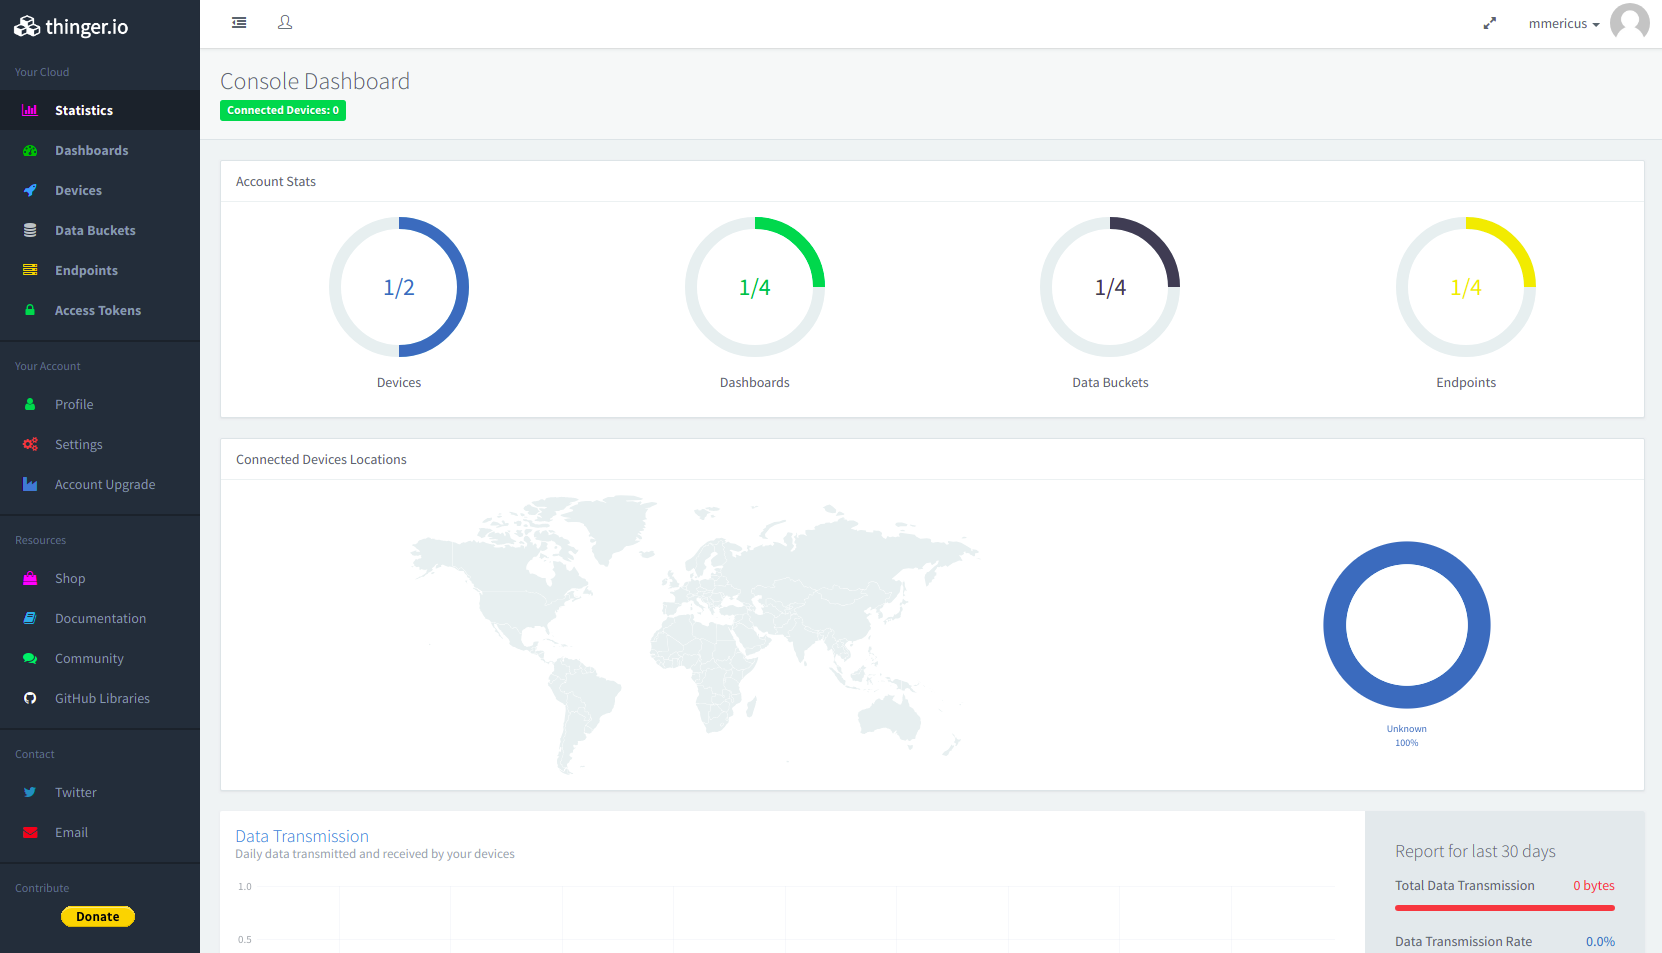
\includegraphics[width=0.85\textwidth]{thinger}
\end{figure}

Platforma je přizpůsobena práci v real-time režimu, kdy je možné například sledovat vývoj vlhkosti vzduchu živě, jako je na následujícím obrázku.
\begin{figure}[H]
\caption{Ukázka grafu v thinger.io}
\centering
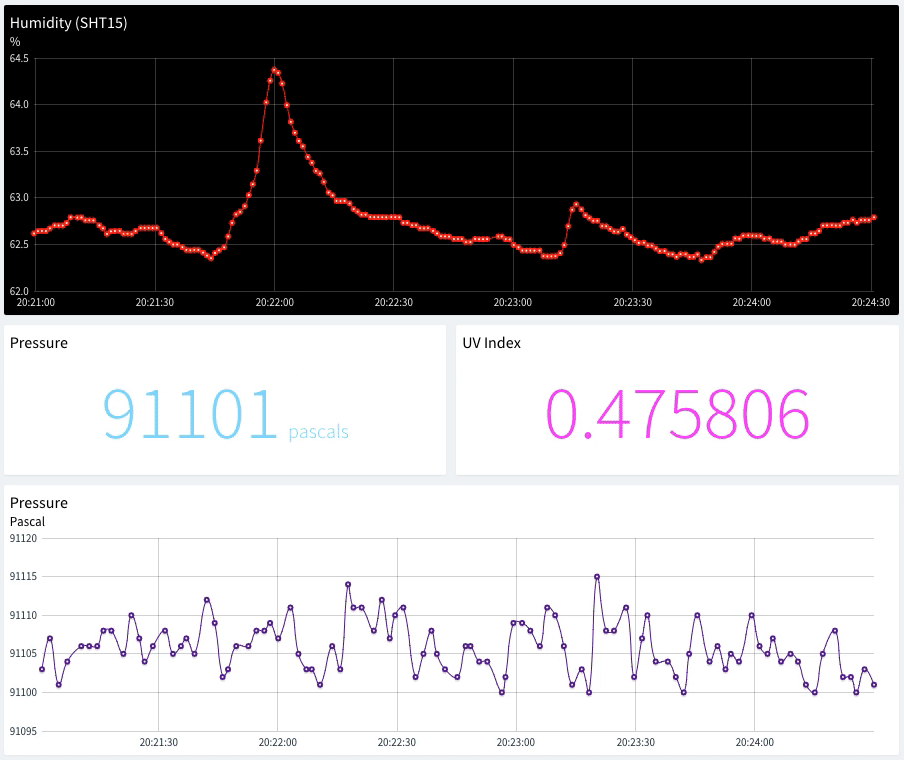
\includegraphics[width=0.85\textwidth]{real-time-iot-dashboards}
\end{figure}

\bigbreak
\newpage
Výhody
\begin{itemize}
 \item Řešení přímo pro shromažďování a prezentaci dat.
 \item Možnost nainstalovat na vlastní servery.
 \item Při zaplacení zákaznická podpora a údržba.
\end{itemize}
\bigbreak
Nevýhody
\begin{itemize}
 \item Zdrojové kódy pro server nejsou dostupné a nelze je tedy modifikovat.
 \item Není možná konverze jednotek.
 \item Podpora pouze JSON formátu.
\end{itemize}

\subsection{IBM Watson IoT Platform}
Po dobu 30 dní je možné využívat platformu v omezeném režimu. Po uplynutí této doby je nutné za platformu platit podle požadované funkcionality a kapacity \cite{ibm}. Platforma umožňuje spravovat senzory a zařízení, rozdělovat je do skupin a mnoho dalšího. Umožňuje zpracovávat data v binárním, textovém a JSON formátu \cite{ibm-format}. 

\begin{figure}[H]
\caption{Ukázka IBM Watson}
\centering
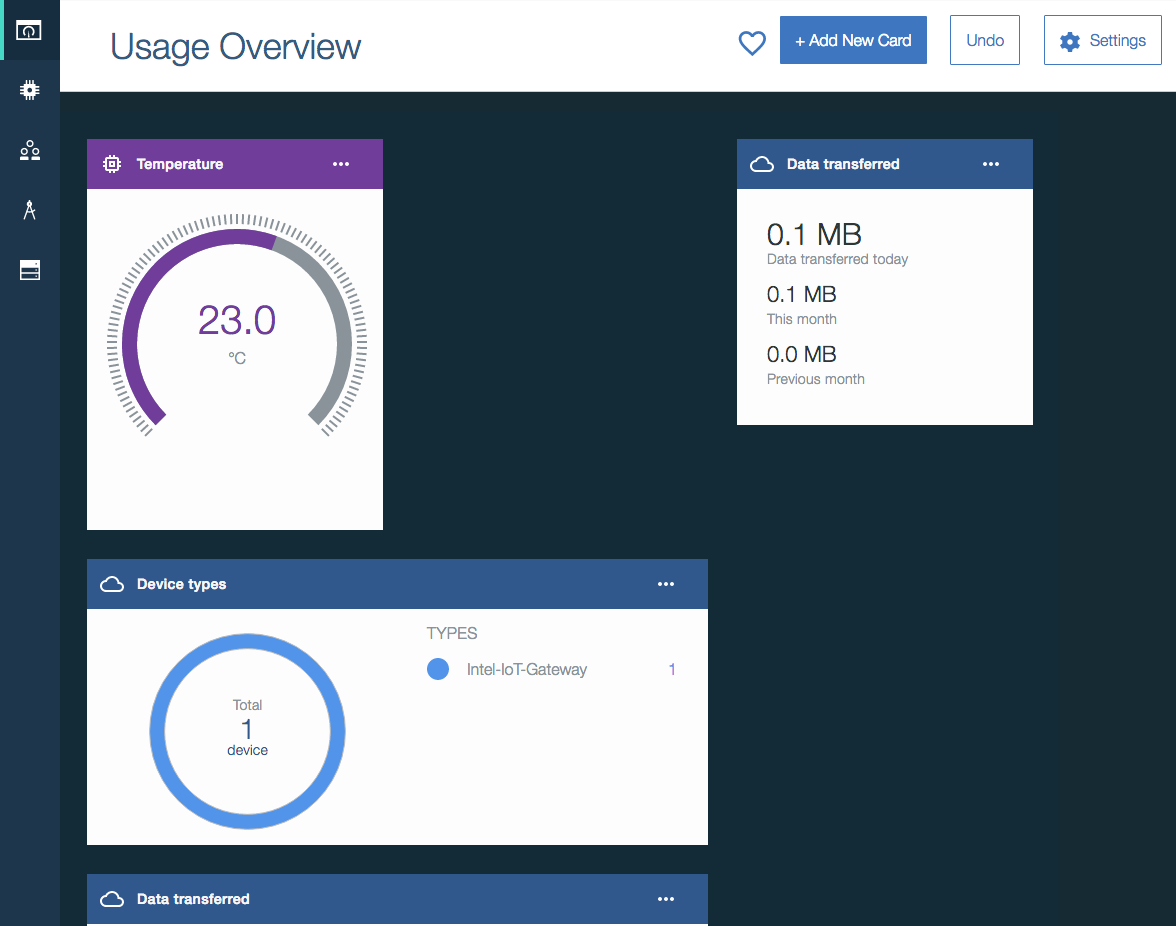
\includegraphics[width=0.85\textwidth]{ibm-temperature}
\end{figure}

\bigbreak
\newpage
Výhody
\begin{itemize}
 \item Umožňuje zpracovávat více formátů (JSON, binární a textový) \cite{ibm-format}.
 \item Udržovaná platforma od známé a stabilní společnosti.
 \item Poskytování široké funkcionality v oblasti IoT. Nezaměřuje se pouze na senzory, ale i na ostatní zařízení.
 \item Lze očekávat neustálý vývoj a rozšiřování.
 \item Zákaznická podpora.
\end{itemize}
\bigbreak
Nevýhody
\begin{itemize}
 \item Placená služba.
 \item Nelze volně rozšiřovat a modifikovat.
\end{itemize}

\subsection{Amazon}
Po dobu 12 měsíců je možné platformu zdarma používat v omezeném režimu. Po uplynutí této doby se platí za provoz, kapacitu a funkcionalitu, která převyšuje zdarma poskytované služby \cite{aws}. Umožňuje přidávat senzory a ostatní zařízení do skupin a spravovat je. Data jsou zpracovávána v JSON formátu \cite{aws-works}.
\bigbreak
Výhody
\begin{itemize}
 \item Udržovaná platforma od známé a stabilní společnosti.
 \item Poskytování široké funkcionality v oblasti IoT. Nezaměřuje se pouze na senzory, ale i na ostatní zařízení.
 \item Lze očekávat neustálý vývoj a rozšiřování.
 \item Zákaznická podpora.
\end{itemize}
\bigbreak
Nevýhody
\begin{itemize}
 \item Placená služba.
 \item Nelze volně rozšiřovat a modifikovat.
 \item Neumožňuje zpracovávat jiný formát než JSON \cite{aws-works}.
\end{itemize}

\newpage

\subsection{Azure IoT Hub}
Tato platforma umožňuje zdarma vyzkoušení oblíbené funkcionality po dobu 12 měsíců. Po dovršení této doby je placená \cite{azure}. Podobně jako předešlá korporátní řešení umožňuje širokou funkcionalitu v oblasti IoT od její správy až po prezentaci dat. Podporuje však pouze JSON formát pro zpracování dat ze senzorů.
\bigbreak
Výhody
\begin{itemize}
 \item Udržovaná platforma od známé a stabilní společnosti.
 \item Poskytování široké funkcionality v oblasti IoT. Nezaměřuje se pouze na senzory, ale i na ostatní zařízení.
 \item Lze očekávat neustálý vývoj a rozšiřování.
 \item Zákaznická podpora.
\end{itemize}
\bigbreak
Nevýhody
\begin{itemize}
 \item Podporuje pouze JSON formát pro zpracování.
 \item Placená služba.
 \item Nelze volně rozšiřovat a modifikovat.
\end{itemize}

\begin{table}[H]\centering
	\caption{Shrnutí rešerše}\label{tab:shrnuti}
\begin{tabular}{ |p{2.5cm}||p{2.5cm}|p{3.5cm}|p{2.6cm}|  }
 \hline
 Platformy & Podporované formáty & Cenová dostupnost & Volně dostupné zdrojové kódy  \\
 \hline
 \hline
 Thinger & JSON & Zdarma (při použití vlastního hardware) jinak placené & Ne \\
 \hline
 IBM Watson & JSON, textový a binární & Placené & Ne \\
 \hline
 Amazon & JSON & Placené & Ne\\
 \hline
 Azure IoT Hub & JSON & Placené & Ne \\
 \hline
\end{tabular}
\end{table}
\newpage
\section{Závěr}
Žádné z nalezených řešení neposkytuje požadovanou funkcionalitu jako open-source a jejich plná verze je dostupná pouze za poplatek. Některé z nich umožňují zdarma jejich využívání v omezeném režimu. Jiné zase neposkytují potřebné funkcionality v oblasti zpracování dat. Tato práce se bude zabývat hlavně zpracováním dat IoT senzorů různých formátů a bude poskytována jako open-source. Každý si bude moci aplikaci nainstalovat na vlastní server a volně ji modifikovat. 

\section{Cíl práce}
Kombinací zadání s provedenou analýzou bylo rozhodnuto, že výsledná aplikace musí splňovat následující body.
\begin{itemize}
  \item Měla by mít webové prostředí.
  \item Volně dostupná.
  \item Snadno modifikovatelná.
  \item Komunikovat pomocí HTTP protokolu a zpracovávat požadavky ze senzorů nebo jiných platforem z oblasti IoT.
  \item Mít uživatelský systém umožňující správcům nastavovat a řídit aplikaci a uživatelům zobrazovat data.
  \item Umožňovat vkládat a spravovat senzory.
  \item Umožnit vytvářet metriky a jednotky.
  \item Umožnit definici zpracování příchozích požadavků dle typů formátů (text, JSON, binární).
  \item Umožnit zanášení senzorů do mapy.
  \item Zobrazovat data ve grafu.
  \item Možnost exportovat data do CSV nebo podobného formátu.
  \item Data budou zobrazena jen uživatelům, kteří dostanou oprávnění.
  \item Ovládání aplikace pomocí interaktivního UI.
\end{itemize}


\chapter{Internet of things}\label{textcompr}
Internet of things (Internet věcí) je nastupující trend digitalizování nejrůznějších fyzických zařízení, která jsou vybavena senzory, elektronikou,  softwarem a síťovými prvky. Tato zařízení dokážou mezi sebou komunikovat a vyměňovat si data. Využívají se pro optimalizaci procesů a pro výzkum.
	\section{Typy senzorů}
V organizacích a průmyslu se používá celá řada typů senzorů. Každý z těchto senzorů snímá různé metriky \cite{iot-types}.
\begin{itemize}
  \item Teplotní senzory -
Zařízení používané k měření tepelné energie, což umožňuje detekovat fyzické změny v teplotě konkrétního zdroje energie a poskytuje tyto údaje zařízení nebo uživateli.
  \item Senzory pro měření tlaku - Zařízení, které snímá tlak a konvertuje ho do elektrického signálu. Jeho síla záleží na úrovni nasnímaného tlaku.
  \item Senzory měření kvality vody - Tento typ senzoru slouží k měření kvality vody v potrubí, vodních zdrojích, atd. Senzory se dále dělí podle toho, jak a co ve vodě v rámci její kvality sledují.
  \item Senzory pro měření koncentrace chemických látek - Tyto senzory jsou používány v nejrůznějších odvětvích. Jejich hlavním cílem je pozorovat chemické změny (například ve vzduchu). Výsledky mohou pomáhat sledovat prostředí ve velkých městech a chránit tak obyvatelstvo.
  \item Senzory pohybu - Elektrické zařízení pro snímání fyzického pohybu. Pohyb jakéhokoliv objektu nebo člověka je převáděn na elektrický signál. Lze využít například pro zajištění bezpečnosti.
  \item Gyroskopy - Senzor detekující úhel a rychlost, jakou je vykonáván pohyb.
  \item Akcelerometr - Senzor využívající se k měření fyzického zrychlení objektu, které bylo způsobeno nějakou inicializační silou. To je poté převedeno opět na elektrický signál.
  \item IR senzory - Tento senzor slouží k měření infračerveného záření, které vyzařují okolní objekty. Lze pomocí něho snímat tepelnou energií, kterou vyzařují objekty.
  \item Senzory kouře - Snímají koncentraci kouře v prostředí. Používají se v průmyslu i v oblasti bezpečnosti běžného života (například v domácnosti). Při detekci určité koncentrace lze spouštět bezpečnostní mechanismy jako například zavolání pomoci.
   \item Obrazové senzory - Jsou využívány k převádění obrazu na elektrický signál. Používají se v kamerách, v lékařství, ve vybavení pro noční vidění. 
  \item Senzory vlhkosti - Sledují množství vodní páry obsažené ve vzduchu nebo jiných plynech.
  \item Optické senzory - Měří množství světelných paprsků a převádí je na elektrický signál, který lze snadno číst uživatelem nebo zařízením.
\end{itemize}
	\section{Komunikace}
Senzory se dále liší ve způsobu komunikace.
\begin{itemize}
  \item Cellular
  \item Wifi
  \item NFC
  \item Bluetooth
  \item Z-Wave
  \item Zigbee
  \item RFID
  \item Smartdust
  \item MEMS
  \item TCP/IP
  \item HAN
\end{itemize}
\chapter{Návrh řešení a použité technologie}\label{textcompr}
Tato kapitola popisuje návrh řešení a technologie, pomocí kterých bude tento návrh implementován.

	\section{Návrh řešení}
	Dle cíle práce má být zhotovena aplikace, která bude mít dvě hlavní funkce. První bude shromažďování dat ze senzorů a jejich ukládání do databáze. Druhá hlavní funkce je filtrování těchto dat a jejich prezentace.
	
	Na základě cíle práce bylo rozhodnuto, že pro komunikaci pomocí HTTP protokolu je vhodná architektura REST. REST je sada pravidel a principů, které pokud jsou dodržovány, umožní dosáhnutí dobrého designu a interoperability systému \cite{rest-about}. V REST architektuře se přistupuje k resource (zdroji) pomocí HTTP metod GET, PUT, PATCH, DELETE, POST. Každý zdroj je identifikován pomocí URI.
	
	 Z důvodů škálovatelnosti výkonu a lepší údržby kódu bylo rozhodnuto, že bude lepší mít dvě rozdělené aplikace. První aplikace bude shromažďovat a ukládat data, která poté bude jako RESTful API poskytovat frontendové aplikaci. Ta se bude starat o jejich prezentaci. Tímto rozdělením lze také získat větší svobodu při výběru technologií, jelikož nyní není nutné, aby aplikace běžely na stejném fyzickém stroji. Další potencionální výhodou je, že se shromážděná data dají poskytovat třetím stranám.
	
\begin{figure}[h]
\caption{Návrh aplikace}
\centering
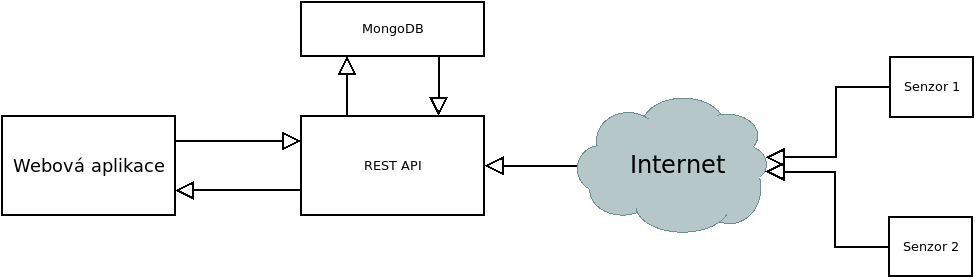
\includegraphics[width=1\textwidth]{diagrams/navrh-aplikace}
\end{figure}


Vzhledem k nastupujícímu trendu bylo rozhodnuto, že obě aplikace budou napsány v JavaScriptu. To umožňuje, aby člověk se znalostí jednoho jazyka byl schopen spravovat obě aplikace. Dále je možné využívat stejné knihovny a zdrojové kódy na obou stranách a vyhnout se tak duplicitám kódu a jejich složité modifikaci. Zároveň se v aktuální době jedná o moderní a velmi podporovanou cestu. RESTful API psané pomocí Node.js totiž umožňuje celou řadu výhod, které budou popsány dále.

Obě aplikace budou využívat flow-type z důvodů větší kvality kódu a menší náchylnosti na nechtěné chyby. Flow-type totiž umožňuje, u jinak dynamicky typovaného jazyku JavaScript, deklarovat i typy. Dodržování jednotného stylu kódu bude hlídat knihovna ESlint.
	
\subsection{Frontend aplikace}
	Jelikož bude aplikace využívána pouze lidmi z technického oboru, tak lze předpokládat, že nebude vytížena častými uživatelskými dotazy na server. Bylo proto rozhodnuto, že bude velmi výhodné napsat aplikaci pomocí Next.js a knihovny React. Next.js vykresluje obsah stránky na straně serveru (server-side rendering). React komponenty budou tedy předvykresleny už tehdy, když uživatel obdrží obsah webové stránky. Tím odpadá nevýhoda Reactu na pomalejších zařízeních, jelikož uživatel musel čekat, dokud prohlížeč neprovede vykreslení. Server side rendering má tedy za výhodu vyšší rychlost na mobilních zařízeních. Nevýhodou je, že se zátěž přesouvá od uživatele na server. Jak již bylo ale řečeno, u aplikace se nepředpokládá vysoká uživatelská zátěž.
	
	Pro bundling je využit Webpack. Jedná se o aktuálně nejpoužívanější a technicky nejlepší variantu. Ke stylování webové stránky bude využita knihovna Bootstrap. Data budou vykreslena v grafech a jednotlivé senzory bude možné zanést do mapy s jejich přesnou polohou.
\subsection{Databáze}
Jako nejlepší databáze k výše zmíněným technologiím bylo zvoleno MongoDB. Lze očekávat veliké množství dat, které bude od senzorů shromažďováno. S tímto nárůstem je tedy nutné počítat a tím pádem i se snižováním výkonu při jejich zpracovávání. MongoDB jako NoSQL databáze dosahuje v tomto případě dobrých výsledků. Je nutné tomu ale přizpůsobit její návrh, jelikož nelze postupovat jako při návrhu relační databáze. 
\subsection{Backend aplikace}
Backend aplikace bude realizována pomocí Node.js a frameworku Express. Data budou zapisována a čtena z MongoDB. Správci bude umožněno vytvářet metriky a jednotky, do kterých budou příchozí hodnoty řazeny. V rámci této práce se vypracují funkce, které dokážou zpracovávat požadavky ve formátech JSON, text a vybrané případy binárních dat. API bude poskytovat endpoint, kam budou moci služby a senzory zasílat svá data. Tato data bude zároveň možné převádět na stejné jednotky a filtrovat podle času vytvoření. Zároveň bude poskytovat stručný přehled a jednoduché statistiky doposud přijatých dat každého senzoru. 
	\section{Uživatelé a jejich oprávnění}
	Uživatelské oprávnění bude víceúrovňové. Na jedné straně budou správci, kteří budou spravovat nastavení (senzorů, metrik, ostatních uživatelů a formáty příchozích dat), a na druhé straně uživatelé, kteří budou sledovat nashromážděné výsledky. Každý uživatel by však měl vidět pouze ta data, ke kterým mu dá správce oprávnění. Toto oprávnění bude ověřováno na obou stranách, tzn. frontendovou aplikací i API. Ověření bude realizováno pomocí tokenu, které API poskytne po přihlášení a které bude frontend aplikace posílat spolu s požadavky, které ho budou vyžadovat.
	
\begin{figure}[h]
\caption{Struktura aplikace}
\centering
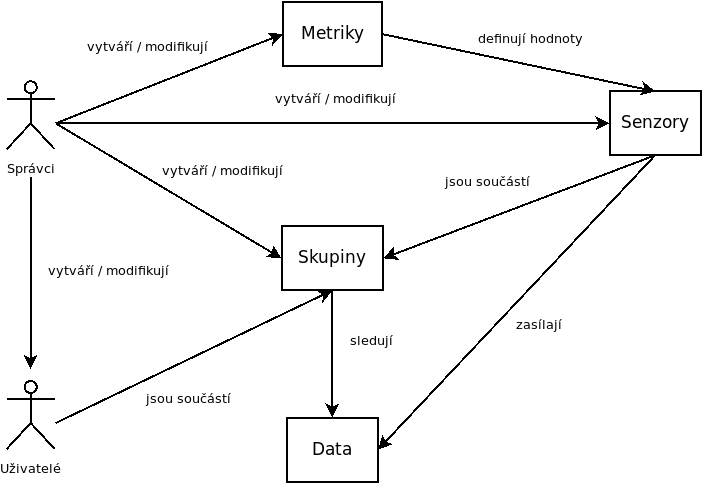
\includegraphics[width=0.95\textwidth]{diagrams/users}
\label{fig:users}
\end{figure}
\newpage
\section{Použité technologie}
	\subsection{Node.js}
	Node.js je framework sloužící k psaní JavaScriptového kódu mimo prostředí prohlížeče. Node.js prostředí umožňuje přístup k různým systémovým funkcím jako přístup k souborům a síťovým prvkům (viz obrázek \ref{fig:nodejs}). Je postaven na engine V8 pro Chrome. V dnešní době je Node.js populární k psaní serverové části aplikací reagujících na I/O události. Node.js všechna data zpracovává po chunkách, a tudíž nikdy žádná neukládá do bufferu \cite{nodejs}.

\begin{figure}[h]
\caption{Důležité části Node.js \cite{nodeimg}}
\centering
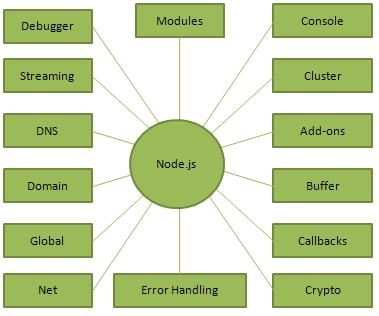
\includegraphics[width=0.9\textwidth]{nodejs_concepts}
\label{fig:nodejs}
\end{figure}

\newpage
	\subsection{Next.js}
Next.js je univerzální framework bežící na serveru i v prohlížeči. Slouží k psaní React aplikací, které jsou vykresleny už na straně serveru (server-side rendering). Na serverové straně Next.js využívá Node.js a framework Express.js.

V klasickém případě přijde uživateli webový obsah, do kterého se následně vykreslí všechny React komponenty. Mezitím je ale uživatel nucen čekat. S server-side renderingem však uživateli přijde již vykreslená webová stránka a on vidí příslušné komponenty hned, jak se stáhne počáteční obsah. Poté dojde k inicializaci Reactu i na straně prohlížeče, ale to už uživatel přímo nevidí. 

To spatřuje výhodu u pomalejších zařízení, která se dostanou k počátečnímu obsahu rychleji. Jednou z nevýhod ale je pochopitelně nutnost většího výkonu na straně serveru.
	\subsection{MongoDB}
MongoDB je dokumentově orientovaná multiplatformní NoSQL databáze. Dokumenty jsou psány ve formátu BSON, který vychází ze známého formátu JSON. Oproti tradičním relačním databázím podporuje dynamické databázové schéma. Zodpovědnost za toto schéma je totiž většinou ponechána na aplikační logice. Při přidání nového atributu máme dvě možnosti. První je, že se musíme spokojit s datovou heterogenitou a řešit problém pomocí aplikační vrstvy. Druhá možnost je doplnit zbývající záznamy o nový atribut, což ale může být výpočetně velmi náročné u mnoha záznamů. 

U MongoDB se musí vývojář oprostit od technik používaných při návrhu relačních databází, protože v případě MongoDB je normalizace databáze kontraproduktivní. Přílišná normalizace vede k více databázovým dotazům a ty jsou zde časově náročnější \cite{mongodb}.
\bigbreak
Výhody:
\begin{enumerate}
\item Flexibilní schéma - Na rozdíl od relačních databází je \textit{schema-less}, což usnadňuje situaci v některých případech.
\item Škálovatelnost - Rychlost čtení lze jednoduše škálovat pomocí replik (více serverů obsahujících stejná data). Zápis lze škálovat pomocí shardingu (rozdělení specifických dat mezi více serverů).
\item Rychlost - Oproti relačním databázím dosahuje MongoDB lepších  výkonnostních výsledků, pokud jsou dodržena pravidla při jeho návrhu jako například denormalizace.
\end{enumerate}
\newpage
Nevýhody:
\begin{enumerate}
\item Flexibilní schéma - Přesouvá zodpovědnost z databáze na aplikaci a programátora.
\item Složitější dotazování (absence JOIN, atd.).
\item Neumožňuje transakce.
\item Velikost - Kvůli optimalizaci rychlosti dochází často k duplicitám dat.
\end{enumerate}
	\subsection{CircleCI}
	Webová platforma pro realizaci continuous integration a continuous delivery. Lze velmi jednoduše propojit s GitHub, na kterém jsou i obě aplikace této diplomové práce. CircleCI nabízí již připravené docker obrazy, ze kterých si stačí pouze vybrat podle používané technologie.

Continuous integration slouží k urychlení vývoje a udržení kvality kódu. Při propojení s GIT repositářem si platforma vytvoří build, na kterém provede testy a ověří jeho správnost. V případě této práce spustí testy aplikace (integrační a unit testy), ESlintu a Flow. Pokud celý tento proces proběhne v pořádku, tak dojde k nahrání nové verze aplikace na produkční nebo testovací prostředí (continuous delivery).

\begin{figure}[h]
\caption{Průběh CI u aplikace}
\centering
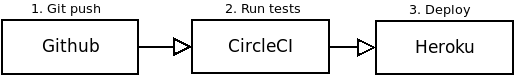
\includegraphics[width=0.9\textwidth]{diagrams/circleci}
\end{figure}
	\subsection{Yarn}
	Yarn je alternativa k npm. Nabízí výhody jako například yarn.lock (v nejnovější verzi npm již existuje také), kdy má vývojář jistotu, jaká verze knihoven bude nainstalovaná na produkční prostředí. Další z výhod je offline cache. Při instalaci knihoven pomocí \textit{yarn install} se tyto balíčky uloží na disk a při jejich opětovné instalaci se už nemusí znovu stahovat.
\newpage
\section{Použité knihovny}
	\subsection{React}
	Dnes velmi populární knihovna pro vytváření uživatelských rozhraní v JavaScriptu. Její největší přínos je specifická manipulace s DOMem. DOM je zjednodušeně řečeno stromová reprezentace komponent, které uživatel vidí v prohlížeči a navíc definuje metody pro manipulaci s ním. Častá manipulace s DOMem může vést ke zpomalení aplikace a právě tento problém pomáhá řešit React. Ten programátora odstiňuje od práce s ním tak, že si vytváří svůj vlastní virtuální DOM, který pomocí různých specializovaných technik porovnává a hledá rozdíly, které pak co nejefektivnějším způsobem aktualizuje \cite{react}. Používáme-li React nebo JSX (templatovací jazyk používaný v Reactu), tak nesmíme nikdy zapomenout React naimportovat na začátku souboru. React se dnes používá velmi často spolu s knihovnou Redux.
	\subsubsection{Props a State}
	 Stav komponenty v Reactu můžeme definovat pomocí \textit{props} a \textit{state}. \textit{State} je vnitřní stav komponenty, do kterého se můžou vkládat libovolná data. Tento \textit{state} se mění pomocí funkce \textit{setState()}. 
	 
	 Pokud komponenty do sebe vnořujeme, tak je potřeba mezi nimi předávat informace. K tomu slouží právě \textit{props}, které ale lze předávat pouze skrz komponenty ze shora dolů. Potomek jej nemůže tedy využít k zaslání dat svému rodiči. Tento problém však jde vyřešit pomocí callback funkcí, které potomek zavolá.
\subsubsection{Lifecycle metody}
Pomocí lifecycle metod můžeme kontrolovat, co se s komponentou děje po celý její životní cyklus (od pre-mount do unmount). Každá z následujících metod se liší v čase, kdy jsou volány (viz obrázek \ref{fig:react-lifecycle}).
\begin{enumerate}
\item static getDerivedStateFromProps - Modifikuje \textit{state} na základě nově příchozích \textit{props} před vykreslením.
\item shouldComponentUpdate -  Metoda, která určuje, zda dojde k překreslení (vrací \textit{true}, nebo \textit{false}).
\item render - Metoda vykreslující komponentu.
\item componentDidMount - Metoda volaná hned po prvním vykreslení.
\item componentDidUpdate - Volaná po každém překreslení komponenty.
\item componentWillUnmount - Metoda volaná před zničením komponenty.
\end{enumerate}
\begin{figure}[h]
\caption{React lifecycle metody \cite{react-lifecycle-img}}
\centering
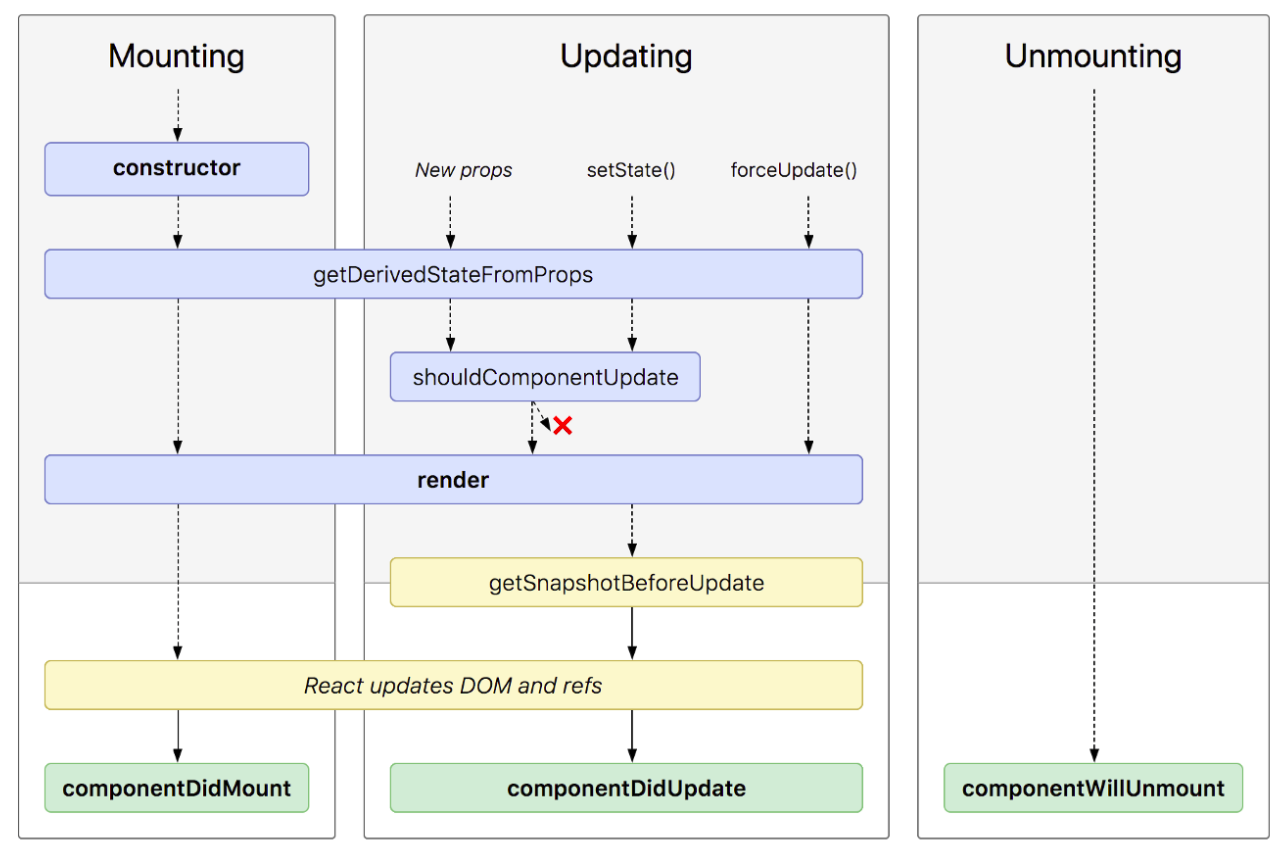
\includegraphics[width=0.9\textwidth]{react-lifecycle}
\label{fig:react-lifecycle}
\end{figure}
	\subsubsection{Vykreslování}
Každá komponenta má jako jedinou povinnou metodu \textit{render}. Tato metoda definuje, co bude vykresleno. Vykresleny můžou být jiné komponenty nebo HTML tagy. Kdy bude komponenta znovu vykreslena, závisí na jejím typu, ale po většinou je znovu vykreslena po každém použití funkce \textit{setState} nebo pokud přijdou nové \textit{props}. Toto chování však závisí na typu komponenty a implementaci \textit{componentShouldUpdate}. React umožňuje vytvářet tři typy komponent:  
\begin{enumerate}
\item Statefull komponenta - Je překreslena po každé změně stavu (\textit{state} a \textit{props}). Metoda \textit{componentShouldUpdate} vždy vrací true (pokud není předefinovaná).  
\item Stateless komponenta - Nemá vnitřní stav, řídí se pouze změnami v \textit{props}.
\item Pure komponenta - V \textit{componentShouldUpdate} se provádí mělké porovnávání aktuálních a nadcházejících stavových objektů. Díky tomu se překreslení neprovádí vždy, jako tomu je u klasické komponenty, ale jen když se \textit{state} nebo \textit{props} liší. Tyto objekty pochopitelně nemohou mít složité vnořené struktury.
\end{enumerate}
\newpage
\subsection{Redux}	
Redux je JavaScriptová knihovna určená pro správu stavu (\textit{state}) aplikace. Lze ho chápat jako aktuální stav aplikace od jejího počátku spolu se všemi změnami, které byly v jejím průběhu provedeny \cite{react-redux}. Způsob manipulace se stavem aplikace lze popsat pomocí následujícího obrázku.\bigbreak
\begin{figure}[h]
\caption{Redux}
\centering
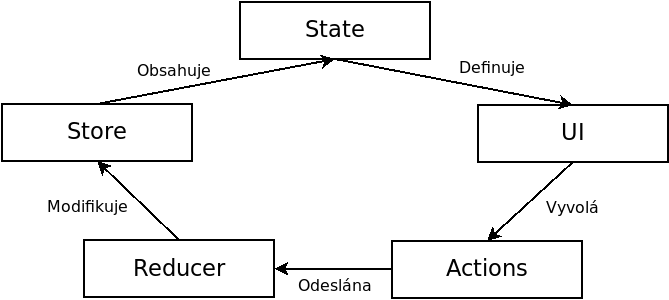
\includegraphics[width=0.9\textwidth]{diagrams/redux}
\end{figure}
Jak je naznačeno na obrázku, tak veškerá modifikace \textit{statu} se provádí pomocí akcí, které reducer přijímá. Reducer určuje, jak se stav aplikace změní po vyvolání specifické akce. Všechny tyto modifikace by měly být imutabilní z důvodů správného překreslování komponent a správného fungování knihovny. Další důležitou částí Reduxu je store. Store je objekt obsahující celý strom stavů a několik řídících funkcí.
	\subsection{Boostrap 4}
	Bootstrap je sada nástrojů pro vývoj webových aplikací. Ulehčují programátorovi práci v oblasti UI a webdesignu. Bootstrap totiž disponuje celou řadou šablon, připravených komponent (například pro formuláře) a animací. Vývojář při jeho využívání nepoužívá klasické CSS styly, ale pouze již definované CSS třídy. Některé jeho funkce jsou stále plně funkční pouze s knihovnou jQuery. Nejnovější verze Bootstrapu (verze 4) je psána v jazycích Sass a JavaScript.
	\subsubsection {Sass}
	Je kompilovaný jazyk rozšiřující syntaxi CSS o celou řadu dalších prvků jako proměnné, podmínky, cykly a mixin. Jeho hlavní výhodou oproti CSS je, že zpřehledňuje kód a šetří čas \cite{sass}.		
	\subsection{Lodash}
	Funkcionální knihovna, která obsahuje mnoho pomocných funkcí pro zpracování polí a objektů. Tyto funkce jsou velmi užitečné při filtrování a grupování dat podle určitých podmínek. Další přidanou hodnotou je, že se funkce dají composovat.
	
	\subsection{Recharts}
	Důležitou funkcionalitou frontend aplikace je zobrazení dat v grafu. Knihovna Recharts poskytuje celou řadu grafů, které jsou napsány jako React komponenty. To má za výhodu snadné modifikování vykreslovaných dat a pomocí již implementovaných animací a designových prvků tak může poskytovat příjemný uživatelský dojem a užitečné funkcionality.

	\subsection{React Google Maps}
	Jednotlivé senzory bude možné zanášet do mapy. Nejrozšířenější a funkcionálně nejbohatší řešení poskytuje Google Maps Platform \cite{google-maps-platform} a jejich implementace pro React s názvem React Google Maps. Pro jejich využívání je však potřeba API klíč, který je poskytován za poplatek. Při vývoji je však možné využít vývojářský klíč. Knihovna umožňuje na základě koordinát (zeměpisné šířky a délky) zanášet na mapu značky, které budou v případě této aplikace reprezentovat právě senzory. 
	
	Google Maps dále umožňují rozšířenou geolokaci na základě názvu objektu, včetně hledání známých míst. Tato funkcionalita ale není v prvotní verzi této práce využita.
	
	\subsection{Mapbox}
Z důvodu poplatků za používání Google Maps Platform je použita i další alternativa a to Mapbox \cite{mapbox}. Ten na rozdíl od Google Maps poskytuje zdarma token na 50 000 zobrazení za měsíc. Správce aplikace se může sám rozhodnout, kterou z platforem používat. Jaká mapa bude použita, bude rozhodnuto na základě toho, jaký API klíč správce při instalaci aplikace zadá.

Používání této platformy umožňuje knihovna \textit{React map gl}, která opět obsahuje připravené React komponenty.
\chapter{RESTful API}
Tato část se věnuje implementaci RESTful API, jehož funkcionalita byla popsána v předešlých kapitolách. Jak bylo naznačeno, toto API je implementováno pomocí frameworku Express a využívá MongoDB databázi. Vývoj probíhal v postupných krocích, které budou v této kapitole popsány.
\section{Prostředí}
Nejprve je nutné nastavit počáteční prostředí. Jako první je třeba nainstalovat všechny potřebné knihovny. Zde je výčet s popisem těch nejdůležitějších z nich:

\begin{enumerate}
\item Babel - JavaScriptový compiler používaný k převedení různých dosud plně nepodporovaných funkcí a syntaxe na jednotnou a podporovanou podobu.
\item Chai - Knihovna pro testování JavaScriptových aplikací. Obsahuje všechny potřebné funkce k psaní unit testů a integračních testů.
\item ESlint - Nástroj pro udržování kvality kódu. Stará se o dodržování pravidel jeho vzhledu a struktury jako například délky řádků a odsazení. Umožňuje definování vlastních pravidel, či využívání pravidel třetích stran.
\item Flow - Rozšíření syntaxe umožňující v dynamicky typovaném JavaScriptu deklarovat typy. Nástroj flow-bin zároveň ověřuje jejich dodržování napříč kódem.
\item Istanbul - Nástroj pro zjišťování, jak je kód pokryt testy.
\item Mocha - JavaScriptový framework běžící na Node.js a v browseru pro asynchronní testování.
\item Nodemon - Nástroj usnadňující vývoj v Node.js. Restartuje server po každé změně kódu.
\item Prettier - Automaticky formátuje kód podle vybraných pravidel.
\item Bcrypt - Šifrovací knihovna, která je použita k šifrování hesel.
\item Body-parser - Middleware pro Node.js používaný k extrakci obsahu příchozích požadavků.
\item Express - Framework pro Node.js, který obsahuje mnoho funkcí ulehčujících vývoj webových aplikací. 
\item Lodash - Knihovna poskytující celou řadu funkcí pro usnadnění práce programátora. Zároveň podporuje funkcionální paradigma.
\item Mongoose - Knihovna umožňující práci s MongoDB v Node.js.
\item Morgan - Slouží k logování HTTP požadavků v Node.js.
\item Passport - Autentizační middleware pro Node.js. Obsahuje i rozšíření podporující JSON web token autentizaci, která je používána v této práci.
\end{enumerate}

\subsection{Adresářová struktura}
Adresářová struktura odpovídá klasické MVC architektuře. Stěžejní je složka \textit{app} a \textit{tests}. Ve složce \textit{app} se nachází veškerá struktura aplikace a ve složce \textit{tests} všechny integrační a unit testy. Ve složce \textit{configs} budou všechny konfigurační soubory včetně konfigurace pro nastavení MongoDB a tajný klíč pro šifrování atd. Tyto konfigurace se prioritně získávají z proměnných operačního systému a poté z JavaScriptových souborů v podsložce \textit{env} (podle aktuálního prostředí).

Za zmínku stojí složka \textit{.circleci}, která obsahuje konfigurační soubor pro CircleCI. Zde jsou nastaveny Node.js a MongoDB docker obrazy, které jsou potřeba k otestování a zprovoznění aplikace. Dále jsou zde definovány dvě workflow, první je testování aktuálního buildu, kdy se spustí Flow, ESlint a testy. Pokud vše proběhne v pořádku, tak se spustí druhá workflow, která otestovaný build nahraje na Heroku.
\begin{figure}[H]
	\dirtree{%
		.1 build \DTcomment{výsledný build aplikace a testů}.
		.1 app.
		.2 config\DTcomment{konfigurace globálních proměnných}.
		.2 controllers\DTcomment{controllery pro zpracování požadavků}.	
		.2 lib\DTcomment{pomocné knihovny}.
		.2 middlewares\DTcomment{middlewary pro zpracování požadavků}.
		.2 models\DTcomment{modely a definice MongoDB dokumenty}.
		.2 routes\DTcomment{routy pro zpracování požadavků}.
		.2 services\DTcomment{pomocné služby}.
		.1 scripts \DTcomment{pomocné skripty }.
		.1 test\DTcomment{složka pro integrační testy a unit testy}.
		.1 consts.js \DTcomment{konstanty}.
		.1 .babelrc \DTcomment{nastavení Babel}.
		.1 server.js\DTcomment{soubor, který spouští a nastavuje aplikaci}.
			}
\end{figure}
\newpage
\subsection{Nastavení Babel}
Jako kompilátor je použit Babel, u kterého je nutné nastavit kompilace flow-type a ECMAScript 6 do podporovaného ECMAScript 2015. Dále byly přidány pluginy umožňující používání modernější syntaxe. Následující zdrojový kód ukazuje Babel konfiguraci uloženou v souboru \textit{.babelrc}.
\begin{lstlisting}
{
  "presets": [
    ["@babel/preset-env",  {
        "targets": {
          "node": "current"
        }   
    }], 
    "@babel/preset-flow"
  ],  
  "plugins": [
    "babel-plugin-dynamic-import-node",
    "@babel/plugin-transform-flow-strip-types",
    "@babel/plugin-proposal-object-rest-spread"
  ]
}
\end{lstlisting}

Dále bylo nutné definovat příkazy, které budou vykonávat buildování a spouštění aplikace. Následující úryvek ze souboru \textit{package.json} zobrazuje definici takových akcí.

\begin{lstlisting}
  "scripts": {
      "heroku-postbuild": "babel app -d build/app",
      "test": "./scripts/test",
      "build": "babel app -d build/app",
      "start": "NODE_ENV=production node build/app/server.js",
      "dev": "nodemon --exec babel-node app/server.js "
    },  
\end{lstlisting}

Každý z příkazů definovaných v úryvku z \textit{package.json} má specifické funkce a je využit v následujících případech
\begin{enumerate}
\item heroku-postbuild - Skript spuštěný Heroku platformou pro vybuildování aplikace.
\item test - Skript starající se o build aplikace, testů a jejich následné spuštění.
\item build - Vykonává build aplikace do složky \textit{build/app/}.
\item start - Spuštění posledního buildu ze \textit{build/app/}. Tento příkaz je používán pro produkční prostředí.
\item dev - Spuštění nástroje Nodemon, který se využívá na vývojovém prostředí. Aplikaci není nutné po každé změně kódu restartovat.
\end{enumerate}
\newpage
\section{Návrh modelů}
Jako další krok před samotným programováním byl nutný návrh struktury celé aplikační logiky vycházející z obrázku \ref{fig:users}. Bylo nutné navrhnout jednotlivé modely tak, aby splňovaly zadání a aby byly stále aktuální, a to i pokud byl model vnořen do jiného modelu a došlo k jeho modifikaci. Zde je nutné mít na paměti požadavky na optimální MongoDB návrh, kdy se musí programátor vyvarovat přílišné normalizaci. Jako první MongoDB dokumenty (modely) byly navrženy ty, do kterých není nutné vnořovat jiné dokumenty. Všechny následující struktury obsahují automaticky generované unikátní ID.

\subsection{Skupiny}
V zadání je definováno, že je nutné umožnit uživatelům vidět vybraná data ze senzorů, které definuje správce. Řešení tohoto bodu je navrhnuto tak, že samotní správci mají přístup k datům všech senzorů. Uživatelé budou přidělováni do skupin, které budou přidělovány jednotlivým senzorům. Uživatel ve skupině A a B tedy uvidí data senzorů, které jsou ve skupině A nebo B. Dokument skupiny bude mít následující jednoduchou strukturu. 

\begin{figure}[h]
\caption{Databázové schéma skupin}
\centering
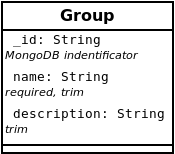
\includegraphics[width=0.40\textwidth]{diagrams/group}
\label{fig:group_schema}
\end{figure}
\newpage
\subsection{Uživatelé}
Nyní už je možné vytvořit uživatelský dokument. Kromě uživatelského jména a hesla bude dokument obsahovat pole identifikátoru skupin, kterých je součástí. Zároveň musíme přidat atribut poskytující informaci o tom, zda se jedná o uživatele, správce nebo libovolnou jinou entitu. Tento atribut je pojmenován \textit{rank} a bude mít číselnou hodnotu. Heslo bude automaticky hashováno pomocí knihovny Bcrypt, kde je pouze potřeba ji povolit u atributu \textit{password} a vložit importovanou knihovnu do uživatelského schématu.


\begin{figure}[h]
\caption{Databázové schéma uživatelů}
\centering
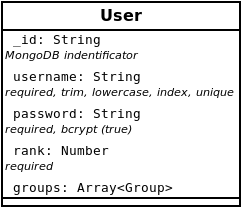
\includegraphics[width=0.50\textwidth]{diagrams/user}
\label{fig:user_schema}
\end{figure}

Aplikace bude mít tři uživatelské role. První role je hlavní správce. Jeho účet bude vytvořen při inicializaci aplikace a je zodpovědný za její provoz. V jeho pravomoci je vytvářet ostatní uživatele a případně další správce. Spolu s ostatními správci může vytvářet metriky, senzory a skupiny. Senzory a uživatelé můžou přiřazovat do skupin, ale sami vidí veškerá data, aniž by těchto skupin byli součástí. 

Každá z těchto tří rolí je reprezentována rankem, který má číselnou hodnotu. Hlavní správce je reprezentován hodnotou nula a ostatní role mají vyšší hodnotu, dle důležitosti v hierarchií. Je-li například dáno, že akce je povolena pouze správcům, tak rank uživatele musí být menší než dva.
\newpage
\subsection{Metriky a jednotky}
Před definicí senzorů a mapperů je nutné definovat metriky a jednotky. Každá metrika by měla mít jednotky. Maximálně jedna jednotka může být označena jako kotevní. Pomocí číselného koeficientu jsou na ni ostatní jednotky převoditelné, což znamená, že se poté dají jednotky převádět i mezi sebou. Tento koeficient bude nepovinný, ale bez něj a kotevní jednotky nebude možné převod provést. Jednotky budou samostatný dokument, který bude vnořen do metrik jako pole.

\begin{figure}[h]
\caption{Databázové schéma metrik a jednotek}
\centering
\subfloat[Jednotky]{{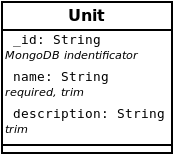
\includegraphics[width=0.40\textwidth]{diagrams/unit} }}%
\label{fig:unit_schema}
\subfloat[Metriky]{{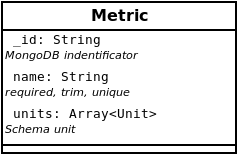
\includegraphics[width=0.55\textwidth]{diagrams/metric} }}%
\label{fig:metric_schema}
\end{figure}

\subsection{Senzor}
Každý senzor nese informaci o svém vlastním výrobním identifikátoru, názvu a popisu. Aby mohl být senzor zobrazen na mapě, tak je třeba dále správci umožnit vyplnit jeho souřadnice \textit{lat} a \textit{lng} (zeměpisnou šířku a délku). Nejdůležitější částí nejen senzoru, ale i celé aplikace, budou mappery, které budou parsovat příslušný obsah z příchozích požadavků. Prozatím pouze určíme, že každý senzor bude obsahovat pole mapperů pro příslušný typ požadavku (JSON, text, atd.). Tato logika bude podrobně vysvětlena v následujících kapitolách.

\begin{figure}[h]
\caption{Databázové schéma senzoru}
\centering
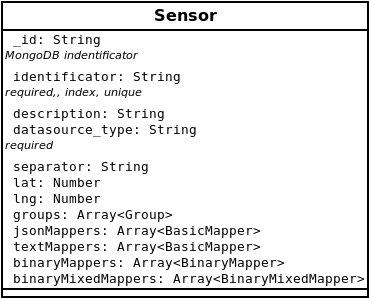
\includegraphics[width=0.80\textwidth]{diagrams/sensor}
\label{fig:sensor_schema}
\end{figure}
\newpage
\subsection{Data}
Tento model bude obsahovat již zpracovaná data ze senzorů. Každá položka dokumentu bude obsahovat hodnotu, ID senzoru, ID metriky, jednotku a statusový příznak. Tento dokument bude obsahovat nejvíc položek a bude používán pro výpis a prezentaci ve frontendové aplikaci.
\begin{figure}[h]
\caption{Databázové schéma dat}
\centering
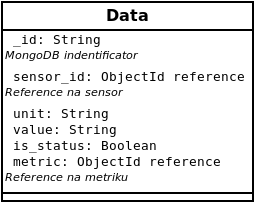
\includegraphics[width=0.50\textwidth]{diagrams/data}
\label{fig:data_schema}
\end{figure}

\section{Routy a controllery}
Nejprve je vhodné vysvětlit, jak funguje vytváření rout a controllerů, jelikož později z toho vychází celá řada middlewarových funkcí, jako například přihlášení. 

\subsection{Routy a controllery v Express}
Routa směruje příchozí požadavky na příslušné akce controlleru. Routa se pomocí frameworku Express vytváří následovně.
\begin{lstlisting}
   app.get(route_path, ...callbacks);
\end{lstlisting}
Pro všechny HTTP metody (GET, POST, PUT, PATCH, DELETE) existují v Express funkce, které jako argumenty přijmou na prvním místě cestu, jakou routa zpracovává a poté libovolný počet callback funkcí. Tyto funkce obdrží jako argumenty \textit{Request}, \textit{Response} a \textit{NextFunction}.

\begin{enumerate}
\item Request - HTTP požadavek extrahovaný do objektu, který obsahuje všechny náležitosti jako metodu, URL parametry, body, atd.
\item Response - Objekt reprezentující budoucí HTTP odpověď. Tento objekt je modifikován a následně odeslán metodou \textit{send}.
\item NextFunction - Metoda říkající, že se má pokračovat v průchodu dalšími callback funkcemi. Bez jejího zavolání je řetězec průchodů ukončen aktuální funkcí.
\end{enumerate}

Tyto callback funkce se dají využít jako middleware, který může například provádět autentizaci nebo jen modifikovat požadavek o další informace. Controller odpovídající na validní požadavek je tedy většinou poslední callback funkce v tomto řetězci.
\begin{lstlisting}
app.get(route_path, ...middlewares, controller.action);
\end{lstlisting}

\subsubsection{Extrakce URL parametrů}
Express provádí extrakci URL parametrů, který se nachází v \textit{PATH} za dvojtečkou. Všechny extrahované URL parametry se poté nachází s totožným názvem v objektu \textit{request.params}, který přichází jako parametr již zmíněných callback funkcí.

\begin{lstlisting}
      GET /users/:parametr -> req.params.parametr
\end{lstlisting}
\subsection{Implementace rout a controllerů}
Jako první je třeba vytvořit controllery s routami pro již navržené modely, aby je mohl uživatel a správce skrz aplikaci vytvářet a číst. Jedná se o controllery pro skupiny, uživatele, metriky a senzory. Tyto controllery sdílí mnoho, mají podobné chování i strukturu. Každý controller obsahuje stejnou sadu základních rout, která se od následující ukázky liší pouze v názvu příslušné entity.
\begin{lstlisting}
      GET /sensors/:_id
      GET /sensors
      PATCH /sensors/:_id
      POST /sensors
      DELETE /sensors/:_id'
\end{lstlisting}
Příslušné akce mají jednoduchou implementaci, kdy se většinou pracuje pouze s Mongoose. Následující ukázka zobrazuje způsob, jakým je implementován proces routování až směrem k akcím controlleru. Routy pro příslušné controllery se nachází ve složce \textit{routes}.
\begin{lstlisting}
// routes/metrics.js

  app.post('/metrics', MetricController.post);
  
// controllers/MetricController.js

  export const post = (req: $Request, res: $Response) => {
    Metric.create(req.body)
      .then(unit => {
        res.status(200).json(unit.toJSON());
      })  
      .catch(err => {
        res.status(400).json(err);
      }); 
  };
\end{lstlisting}

Všechny routy jsou dynamicky importované v souboru \textit{server.js} pomocí knihovny Glob. Glob umožňuje synchronně načítat soubory pomocí patternů.

\begin{lstlisting}
// server.js 

  glob.sync('routes/**/*.js', 
    { cwd: __dirname }).map(filename => {
      import('./'.concat(filename)).then(module => {
        module.default(app);
      }); 
  });
\end{lstlisting}
\newpage
\section{Přihlašování}
Při implementaci přihlašování se používá JavaScriptová knihovna Passport, která poskytuje middleware pro Node.js podporující celou řadu různých strategií přihlašování, a to i přes různé systémy třetích stran, jako například GitHub, Facebook, Google, atd. V této aplikaci se bude používat strategie využívající JSON web token.
	\subsection{JSON web token}
	JSON web token je standard splňující RFC 7519 \cite{rfc}, který se používá k zabezpečení komunikace mezi API a klientem. Bezpečně přenáší informace mezi komunikujícími stranami jako JSON objekt \cite{jwt}. Věrohodnost tohoto objektu může být ověřována, jelikož je podepsán příslušným algoritmem. JWT může být podepsán tajným klíčem, například pomocí HMAC. Passport v JWT objektu uchovává informace identifikující uživatele a čas expirace tokenu. Proces přihlašování při použití JWT lze popsat pomocí následujícího obrázku.
\begin{figure}[h]
\caption{JWT proces}
\centering
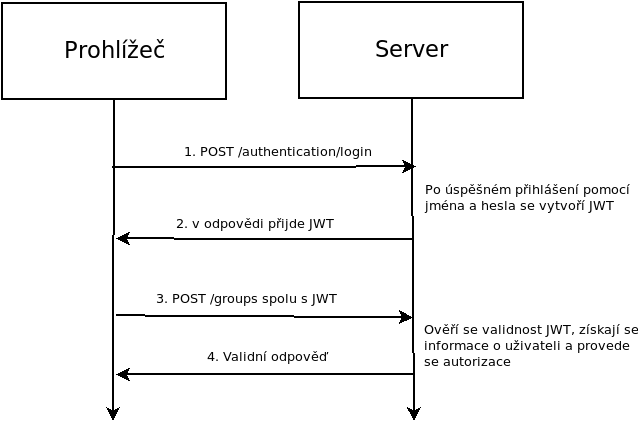
\includegraphics[width=1\textwidth]{diagrams/jwt}
\end{figure}

\newpage
\subsection{Vytvoření tokenu (přihlášení)}
Přihlášení je vyvoláno endpointem s routou \textit{POST /authentication/login}, kde v body je zasláno uživatelské jméno a heslo. Tuto routu zpracovává příslušný controller, který získá uživatele odpovídajícího příslušnému uživatelskému jménu. Knihovna Bcrypt poté provede porovnání hashů hesla z databáze a hesla z požadavku. Pokud je zjištěna shoda, tak se zavolá metoda, která vytvoří JWT. Nejelegantnější umístění této metody je přímo v definici modelu uživatele, protože se poté dá zavolat na každou instanci daného uživatele.

\begin{lstlisting}
// models/User.js

  UserSchema.methods.getJwt = function() {
    const expiration_time = parseInt(config.jwt_expiration);
    return (
      'Bearer ' + jwt.sign(
      	{ user_id: this._id }, 
      	config.jwt_secret, 
      	{ expiresIn: expiration_time }
      )
    );  
  };
 
// controllers/AuthController.js 

   export const login = (req: $Request, res: $Response) => {
    User.findOne(
      { username: req.body.username },
      (error, user) => {
        const isPasswordValid = bcrypt.compareSync(
          req.body.password,
          user.password,
        )
        if (!isPasswordValid)
          return res
            .status(401)
            .send({ auth: false, token: null })
  
        res.status(200).json({
          auth: true,
          token: user.getJwt(),
          username: user.username,
          rank: user.rank,
        })
      }, 
    )
  }



\end{lstlisting}

\newpage
\subsection{Passport strategie}
	Pro používání passport je třeba implementovat vlastní JWT strategii, kde se nastaví, pomocí jaké funkce získat token a jak získat uživatele z informací v něm uložených. K implementaci takovéto funkcionality je potřeba doinstalovat strategií pro JWT s názvem \textit{passport-jwt}.

Získávat token bude podle strategie bearer authentication scheme, které token obsahuje v hlavičce authentication s předponou \textit{bearer}. V překladu toto schéma lze popsat jako "Dát přístup držiteli (bearer) tohoto tokenu"\cite{bearer}.
\begin{lstlisting}
Authorization: Bearer <token>
\end{lstlisting}

Zdrojový kód strategie vypadá následovně. Nejprve se získá token a poté se vloží spolu s \textit{jwt\_secret} (uloženým v konfiguračním souboru) do objektu, pomocí něhož se vytvoří nová passport strategie. Tato strategie pomocí uživatelského identifikátoru, který byl uložen v tokenu, získá existujícího uživatele. Pokud jakýkoliv krok skončí neúspěchem, tak dojde k chybné autorizaci a odeslání příslušné odpovědi.

\begin{lstlisting}
  export default (passport: Passport) => {
    var opts = {};             
    opts.jwtFromRequest = ExtractJwt.fromAuthHeaderAsBearerToken();
    opts.secretOrKey = config.jwt_secret;
  
    passport.use(
      new Strategy(opts, async function(jwt_payload, done) {
        User.findById(jwt_payload.user_id)
          .lean()
          .exec((err, user) => {
            if (err) throw err;
  
            if (user) {        
              return done(null, user);        
            } else {           
              return done(null, false);       
            }                  
          });
      }),
    );
  };
\end{lstlisting}
\newpage
\section{Mappery}
Další důležitou částí aplikace jsou mappery. Jejich úkolem bude mapovat a parsovat data z požadavků příslušným metrikám. Mapper bude sloužit ke zpracování určitého formátu obsahu požadavku. Tato práce se zabývá hlavně zpracováním textového, JSON a binárního formátu reprezentovaného v hexadecimální soustavě.


Každý mapper může obsahovat místo metriky a jednotky statusový příznak \textit{is\_status}. To je booleovská hodnota, která říká, že daná zpracovaná hodnota nese kód, v jakém stavu se senzor nachází nebo proč nemohla dorazit validní data.


Senzor bude mít jeden typ mapperů a bude určen ke zpracování jednoho formátu dat. Každý typ mapperu se bude nacházet v modelu senzoru v poli a každý mapper v tomto poli bude sloužit k nalezení jedné hodnoty.


Pokud přijde požadavek na příslušný endpoint, nejprve je nutné zjistit, o který senzor se jedná, aby byly použity příslušné mappery. To bude probíhat tak, že přijde-li požadavek, tak bude zpracován globálními mappery pro detekci senzoru podle identifikátoru. Zjednodušeně řečeno aplikace bude hledat identifikátor v požadavku na místech, která definuje správce.

\subsection{JSON mapper}
Model mapperu pro JSON bude obsahovat 4 atributy. Cestu k hledané hodnotě, ID metriky, jednotku a statusový příznak. Cesta k požadované hodnotě budou klíče potřebné k dosažení hodnoty oddělené tečkou.
\begin{lstlisting}
{ "key": { "key2": 10 } } => key.key2
{ "key": [{ "key2": 10 }, { "key3": 10 }] } => key[1].key3
\end{lstlisting} 
Schéma takového mapperu bude vypadat následovně:
\begin{figure}[h]
\caption{Databázové schéma JsonMapperu}
\centering
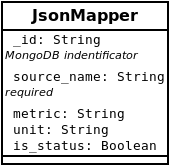
\includegraphics[width=0.40\textwidth]{diagrams/jsonMapper}
\label{fig:jsonMapper_schema}
\end{figure}

\newpage
\subsection{Text mapper}
Textový formát je zasílán v podobě textového řetězce key-value hodnot oddělených separátorem. Separátor je uložen v modelu senzoru. Ke zpracování tohoto formátu je plně postačující schéma mapperu, který byl definován pro JSON formát. \textit{JsonMapper} můžeme tedy přejmenovat na \textit{BasicMapper}, jelikož bude využíván pro svoji univerzalitu více formáty. 

Následující ukázka zobrazuje, jaké hodnoty \textit{source\_name} a \textit{separator} jsou potřeba pro získání hodnoty \textit{val1} klíče \textit{key1} z příslušného řetězce. 
\begin{lstlisting}
key1=val1;key2=val2 => source_name="key1=" separator=";"
\end{lstlisting}
\subsection{Bin mapper}
Na fungování binárního mapperu se lze dívat z mnoha úhlů. Může nám přijít JSON, kde pouze vybraná hodnota bude obsahovat binární data. Další možností je, že nám například přijde \textit{octet-stream} požadavek, který bude kompletně v binární podobě.
V každém případě je tedy v konečném důsledku nutné zpracovat nějaká binární data, ale je nespočetně mnoho způsobů, jak je v požadavku nalézt. Tato aplikace v prvotní verzi bude řešit pouze dva případy. Přijdou-li data v \textit{octet-stream} požadavku nebo v JSON, budou se zpracovávat po bytech, jelikož se zatím věnujeme zpracování hexadecimálního formátu. Z těchto důvodu je tedy nutné, aby měl základní binární mapper následující položky.
\begin{enumerate}
\item Od jakého bytu hodnota začíná.
\item V jakém bytu hodnota končí.
\item Jakou má hodnota metriku a jednotku nebo zda má statusový příznak.
\end{enumerate}

\begin{figure}[h]
\caption{Databázové schéma BinaryMapperu}
\centering
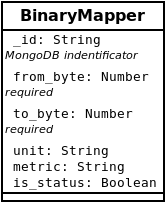
\includegraphics[width=0.35\textwidth]{diagrams/binaryMapper}
\label{fig:binaryMapper_schema}
\end{figure}
\newpage
Za pomoci těchto položek lze získat hodnotu z binárních dat pomocí jednoduchého zpracování řetězce. 
\begin{lstlisting}
parseInt(binaryValue.substr(from_byte, to_byte), 16)
\end{lstlisting}

Zároveň je umožněno tento binární mapper vkládat do jiných mapperů, které budou mít pouze za úkol extrahovat hodnotu z jiného formátu požadavku jako například JSON a zpracování této hodnoty nechají na binárním mapperu. 
\begin{figure}[h]
\caption{Databázové schéma BinaryMixedMapperu}
\centering
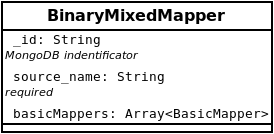
\includegraphics[width=0.60\textwidth]{diagrams/binaryMixedMapper}
\label{fig:binaryMixedMapper_schema}
\end{figure}
\section{Použití mapperů}
Přijde-li požadavek na endpoint \textit{/datasource}, tak je proces zpracování rozdělen do následujících kroků. 
\subsection{Získání senzoru}
Nejprve je požadavek zpracován middlewarem, který se pokusí zjistit identifikátor senzoru pomocí mapperů k tomu určených. Podle \textit{content-type} se však vyberou pouze mappery pro příslušný formát požadavku. Přijde-li požadavek s \textit{content-type json/application}, tak je funkcí \textit{SensorIdParser} zpracován pomocí \textit{IdParseru} pro JSON. Pokud dojde k získání identifikátoru, tak se funkce pokusí nejprve získat senzor podle databázového identifikátoru a pokud senzor nebude nalezen, tak se pokusí vyhledat pomocí atributu \textit{identificator}.
\begin{lstlisting}
if (headers['content-type'] === consts.contentType.JSON) { 
    const sensorIdMapper = await SensorIdMapper.find({
        content_type: consts.contentType.JSON})  
    if (!sensorIdMapper) return null
         
    const sensorId = 
        JsonIdParser(sensorIdMapper, requestBody) 
    const sensor = 
        await Sensor.findOne({identificator: sensorId})   
    if (!sensor) return await Sensor.findById(sensorId)
  
    return sensor

\end{lstlisting}
Poté se nalezený senzor vloží k objektu požadavku pod atribut \textit{sensor} a pokračuje se ve vykování řetězce dalších middlewarů, pokud nějaké jsou, až k samotnému \textit{DatasourceControlleru}. V opačném případě je zaslána odpověď \textit{400 Bad Request}.
\subsection{Získání dat}
	Požadavek je následně controllerem zaslán ke zpracování \textit{DataParseru}, který podle \textit{content-type} a \textit{datasource} atributu, již nalezeného senzoru z předešlého kroku, zvolí správný parser. Atributy \textit{content-type} a \textit{datasource} se ověřují společně, protože binární data mohou přijít i v \textit{content-type} JSON, jak bylo vysvětleno dříve.
	\begin{lstlisting}
if (
  headers['content-type'] === consts.contentType.JSON &&
  sensor.datasource_type === consts.datasource.JSON_BINARY
  ) {
    return JsonBinParser(requestBody, sensor)
  }

\end{lstlisting}
Příslušný parser následně vrátí již rozparsovaná data v poli, ve kterém bude objekt ve formátu Data modelu (navrženého v předešlých kapitolách), který se následně uloží do MongoDB.


\section{Poskytování dat}
Data jsou poskytována oprávněným uživatelům na endpointu \textit {GET /data}. V prvotní verzi aplikace jsou navrhnuty dvě podoby dat, které budou uživateli zaslány.

První data jsou přehledová. Jsou to data specifické metriky a senzoru, která jsou poté vypisována po označení senzoru na mapě, jak je zobrazeno na obrázku \ref{fig:overview}. V tomto detailu se nachází základní informace o senzoru jako jeho identifikátor a popis. Dále jsou zde charakteristiky jeho dat jako minimální a maximální hodnota a průměr. Pro získání těchto dat je nutné provolat endpoint 
\begin{lstlisting}
GET data/overview/:metricId/:sensorId
\end{lstlisting}
\newpage
Jako odpověď poté přijde pole přehledových dat specifické metriky a senzoru. Tato data se ale nejprve převedou na stejnou jednotku. Následující kód vytváří přehled podle popsaných specifikací.

\begin{lstlisting}
  const getOverview = async ( data: Array<Data> ) => {
    const convertedData = await convertValuesUnit(
      data, metricId, unit,
    ) 
    
    const { 
      min, max, sum, numberOfValidItems,
    } = getOverviewData(convertedData)

    return {
      min,
      max,
      mean: getMean(sum, numberOfValidItems),
      unit,
    }
  }

\end{lstlisting}
Jak již bylo řečeno, každá položka obsahuje minimální a maximální hodnotu, průměr a jednotku, ve které jsou tyto hodnoty. To vše je stahováno po každém označení senzoru na mapě z důvodu lepšího výkonu. Jinak by se musela stahovat všechna data na počátku a to by bylo časově náročné.


Druhý endpoint je provoláván s ID senzoru. Jeho výsledkem jsou všechna data, která jsou pro daný senzor uložena.
\begin{lstlisting}
GET /data/:sensorId
\end{lstlisting}
 To je následně exportovatelné do CSV nebo vykresleno v grafu. Endpoint umožňuje zaslat další parametry, které zpřesní nebo modifikují výsledek.


Následující požadavek získá data senzoru určité metriky a případně zkonvertuje na stejnou jednotku (pokud je to možné).
\begin{lstlisting}
GET /data/:sensorId/:metricId?convertUnit=unit
\end{lstlisting}
Tento požadavek pošle data za poslední rok, měsíc, týden nebo den. Akceptuje pouze konstanty \textit {years, months, weeks a days}.
\begin{lstlisting}
/data/:sensorId?lastDate=lastDateUnit
\end{lstlisting}
Všechny zmíněné parametry lze vzájemně kombinovat. Dále je možné požádat o statusová data. To jsou, jak již bylo řečeno, data, která mají místo metriky a jednotky statusový příznak. Díky těmto datům uživatel zjistí, v jakém stavu je senzor nebo zda nenastala nějaká chyba. K získání takových dat je vystaven endpoint 
\begin{lstlisting}
GET /data/:sensorId/status}
\end{lstlisting}

\chapter{Frontend aplikace}
Tato část bude stručně popisovat řešení frontendové aplikace, která využívá API zpracované v předešlé kapitole. Tato aplikace bude zhotovena pomocí frameworku Next.js a knihoven React a Redux. Ke stylování se bude používat Bootstrap navržený speciálně pro React a obsahující i navíc užitečné React komponenty.

\section{Prostředí}
Jak již bylo řečeno, tak k vývoji je použit framework Next.js. To usnadňuje inicializaci a prvotní nastavení projektu, jelikož většina základních konfigurací je již v základním nastavení po jeho instalaci. K získání údajů, jako například URL adresa API, se využívají opět systémové proměnné, ale na rozdíl od API se poté na druhém místě berou ze souboru \textit{.env}.

Oproti API byly použity následující knihovny a pluginy.
\begin{enumerate}
\item babel/polyfill - Poskytuje funkce, které vývojář očekává, že jsou ve všech prohlížečích nativně. Některé funkce, jako například \textit{Promise}, stále nejsou jednotně nativně implementovány napříč všemi prohlížeči.
\item babel/preset-react - Babel preset pro kompilaci Reactu.
\item zeit/next-sass - Jelikož v této aplikaci je použit Bootstrap 4, který je napsán v Sass, tak je nutné stáhnout rozšíření pro Next.js, které bude Sass soubory zpracovávat.
\item axios - Axios je používán ke komunikaci mezi aplikací a RESTful API. Ulehčuje zasílání HTTP požadavků v browseru a Node.js, které se poté zpracovávají asynchronně jako promisy.
\item dotenv - Knihovna umožňující pohodlné načítání proměnných z \textit{.env} souborů spolu se systémovými proměnnými.
\item moment - Moment usnadňuje práci s časem a datumy.
\item Jest - Testovací knihovna.
\item react-test-renderer - Knihovna potřebná pro psaní snapshot testů.
\item next-redux-wrapper - Wrapper pro Next.js integrující Redux do React.
\item react - Knihovna pro psaní UI v JavaScriptu.
\item react-bootstrap - Rozšíření pro React integrující knihovnu pro stylování bootstrap. V této práci je použit nejnovější Boostrap verze 4, který je napsán v Sass.
\item react-google-maps - Pro zobrazení umístění senzorů jsou použity Google mapy. Pro React je možné využít již odladěnou komponentu.
\item redux a react-redux - Správa stavu aplikace.
\item recharts - React komponenty pro vykreslování grafů.
\item redux-thunk - Redux-thunk umožňuje využívat asynchronní akce.
\item universal-cookie - Knihovna usnadňuje práci s cookie.
\end{enumerate}
\subsection{Redux}
Konfigurace Reduxu se bude nacházet v základním souboru \textit{./src/redux.js}. V tomto souboru se budou i shlukovat reducery pomocí funkce \textit{combineReducer}. Akce budou vykonávány asynchronně pomocí knihovny redux-thunk. Jedna z akcí včetně definice návratového typu může vypadat následovně:
\begin{lstlisting}
  type LoginAction =
    | { type: 'LOGIN_PENDING' }
    | { type: 'LOGIN_FULFILLED', username: string }
    | { type: 'LOGIN_REJECTED', payload: ErrorResponse }
  

  export const login = (data: Object) => async ({
    dispatch,
    apiClient,
  }: (ActionDeps) => Promise<LoginAction>) => {
	// implementace  
  }
\end{lstlisting}
\newpage
Každá akce je následně zpracována příslušným reducerem. U každého reduceru se definuje typ daného stavu spolu s inicializačními hodnotami.
\begin{lstlisting}
  export type UserState = {
     // datové typy jednotlivých položek
  }
  const INITIAL_STATE = {
     // počáteční stav  
  }
  
  const reducer = (
     state: UserState = INITIAL_STATE,
     action: UserAction) => 
  {
    switch (action.type) {
      case 'LOGIN_PENDING':
      	// modifikace stavu
      case 'LOGIN_REJECTED':
        // modifikace stavu
      case 'LOGIN_FULFILLED':
        // modifikace stavu
      default:
        return state
    }
  }
  
  export default reducer

\end{lstlisting}
\newpage
\section{Adresářová struktura}
Struktura je přizpůsobena frameworku Next.js, který jednotlivé stránky automaticky zpracovává ze složky \textit{pages}. Výsledný build Next.js ukládá do složky \textit{.next}, která se i automaticky při buildu vytvoří. Stejně jako u API je zde složka \textit{.circleci} s nastavením CircleCI. Samotné zdrojové kódy včetně React komponent se poté nachází ve složce \textit{src}.
\bigbreak
\begin{figure}[H]
	\dirtree{%
		.1 .circleci\DTcomment{konfigurace CircleCI}.
		.1 .next\DTcomment{build aplikace}.
		.1 \_\_tests\_\_\DTcomment{složka pro testy}.
		.1 pages\DTcomment{implementace stránek pro Next.js}.
		.2 \_app.js.
		.2 \_document.js.
		.1 src\DTcomment{složka se zdrojovými kódy}.
		.2 components\DTcomment{zde budou často používané komponenty}.
		.2 libs\DTcomment{externí zdrojové kody jako např. Bootstrap}.	
		.2 helpers\DTcomment{často používané funkce}.
		.2 redux.js\DTcomment{základní Redux soubor}.
		.2 types.js\DTcomment{Definování typů pro Flow}.
		.1 static.
		.1 tests.
		.1 .babelrc\DTcomment{konfigurace Babel}.
		.1 .env\DTcomment{globalní proměnné}.
		.1 .eslintrc.js\DTcomment{konfigurace ESlint pravidel}.
		.1 .prettierrc\DTcomment{definice pravidel pro Prettier}.
		.1 heroku-postbuild.sh\DTcomment{post-build skript pro Heroku}.
		.1 next.config.js\DTcomment{konfigurace Next.js}.
	}
\end{figure}
\newpage
\section{Stránky}
Stránky frontend aplikace převážně reflektují rozvržení controllerů u API. V Next.js má každá stránka soubor ve složce \textit{pages}. URL stránky je dáno názvem souboru. Implementaci stránky \textit{users} najdeme tedy v souboru /\textit{pages/users.js}. Seznam všech stránek této aplikace je následující:

\begin{enumerate}
\item index - Základní stránka, která je také zobrazena nepřihlášenému uživateli.
\item login - Přihlašovací stránka.
\item users - Vytváření a mazání uživatelů, které je přístupné pouze správci.
\item changePassword - Stránka pro změnu hesla.
\item metrics - Správa metrik a jednotek (pouze pro správce).
\item sensors - Správa senzorů a mapperů (pouze pro správce).
\item sensorIdMappers - Správa mapperu pro parsování ID (pouze pro správce).
\item groups - Vytváření a mazání skupin (pouze pro správce).
\item data - Prezentace nashromážděných dat přístupná oprávněným uživatelům.

\end{enumerate}
Pokud chceme všechny stránky rozšířit například o nastavení \textit{favicon.ico} nebo pozměnit základní rozvrstvení HTML stránky, tak je možné využít soubor \textit{/pages/\_document.js}. Tento soubor je v Next.js šablonou pro všechny stránky, do kterého se následně vkládají.

Obdobně funguje i React v Next.js. Každá stránka je JavaScriptový soubor, který obsahuje React komponenty, které jsou vždy vykresleny v souboru \textit{app}, který tvoří Reactovou nejvrchnější vrstvu v Next.js. V tomto souboru se například integruje Redux. V případě této aplikace se zde taktéž kontroluje, zda je uživatel přihlášen.

Pro základní vzhled stránky včetně umístění menu byla vytvořena komponenta \textit{Page}, do které se obalují ostatní komponenty u většiny stránek.
\newpage
\section{Komponenty a jejich organizace}
	Každá stránka má ve složce \textit{app} vlastní podsložku s React komponentami. Každá taková podsložka má také vlastní Redux akce a reducery, které se poté pomocí funkce \textit{combineReducer()} v souboru \textit{redux.js} shluknou dohromady. Většina těchto komponent je psána jako stateless nebo pure, (pokud není vyžadována vlastní implementace funkce \textit{componentShouldUpdate}).
	
	Některé z komponent využívají funkci connect, která mapuje \textit{state} a akce z Reduxu do \textit{props}. Tento proces se však provádí v odděleném souboru, který až posléze pošle všechny tyto \textit{props} příslušné komponentě. To se v této aplikaci dělá z důvodů snadného testování, protože pokud samotná komponenta není připojena na Redux, ale data z něj chodí přes \textit{props} z jiné komponenty, tak je pak možné tyto \textit{props} mockovat a provádět snapshot testy. 
	
Následující příklad ukazuje soubor mapující \textit{state} metriky a akci \textit{getMetrics} z Redux do komponenty \textit{Mapper}. Při testování této komponenty je pak velice snadné tyto hodnoty nahradit vlastními smyšlenými, které budou nezávislé na stavu Reduxu.
\begin{lstlisting}
import { connect } from 'react-redux'
  import Mapper from './Mapper'
  import { getMetrics } from '../../metric/actions'
  
  export default connect(
    ({ metric: { metricList } }) => ({
      isFetching: metricList.isFetching,
      metrics: metricList.metrics,
    }), 
    { getMetrics },
  )(Mapper)
\end{lstlisting}

\section{Prezentace dat}
Jak bylo zmíněno, většina komponent pouze spravuje jednotlivé MongoDB dokumenty a nejsou nijak zajímavé. Dvě komponenty se však liší a plní onu prezentační funkci.

Na stránce pro vizualizaci dat si může uživatel vybrat, zda chce vidět detail senzoru nebo všechny senzory dané metriky. Jelikož lze očekávat větší množství senzorů, tak je k dispozici jednoduchý vyhledávač podle identifikátoru senzoru \ref{fig:sensor_search}.

\begin{figure}[h]
\caption{Ukázka vyhledávače}
\centering
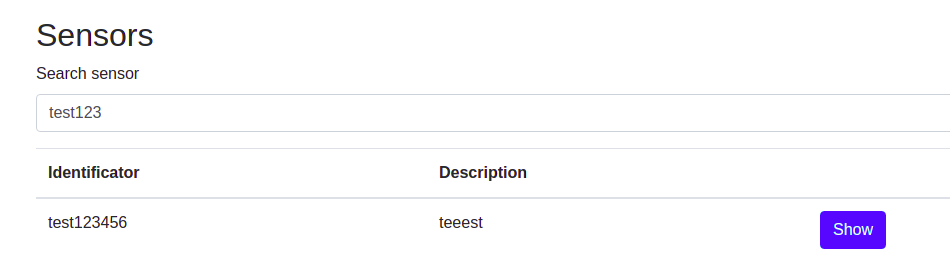
\includegraphics[width=0.95\textwidth]{sensor-search}
\label{fig:sensor_search}
\end{figure}

\newpage
\subsection{Detail senzoru}
První taková komponenta je detail senzoru. Jak lze vidět na obrázku \ref{fig:sensor_graph}, tak na detailu senzoru je k dispozici stažení dat v CSV a filtry, pomocí kterých si uživatel může data vybrat. Pokud to nastavení metriky umožní (data mají kotevní jednotku a jsou validní), tak je vykreslen graf za vybraný časový horizont. Jako poslední se ve spodní části nachází výpis posledních deseti statusů zaslaných senzorem (jejich kompletní výpis je opět stáhnutelný v CSV). K získání dat potřebných k zobrazení této komponenty je využit endpoint \textit{/data/sensorId}.
\begin{figure}[h]
\caption{Ukázka detailu senzoru}
\centering
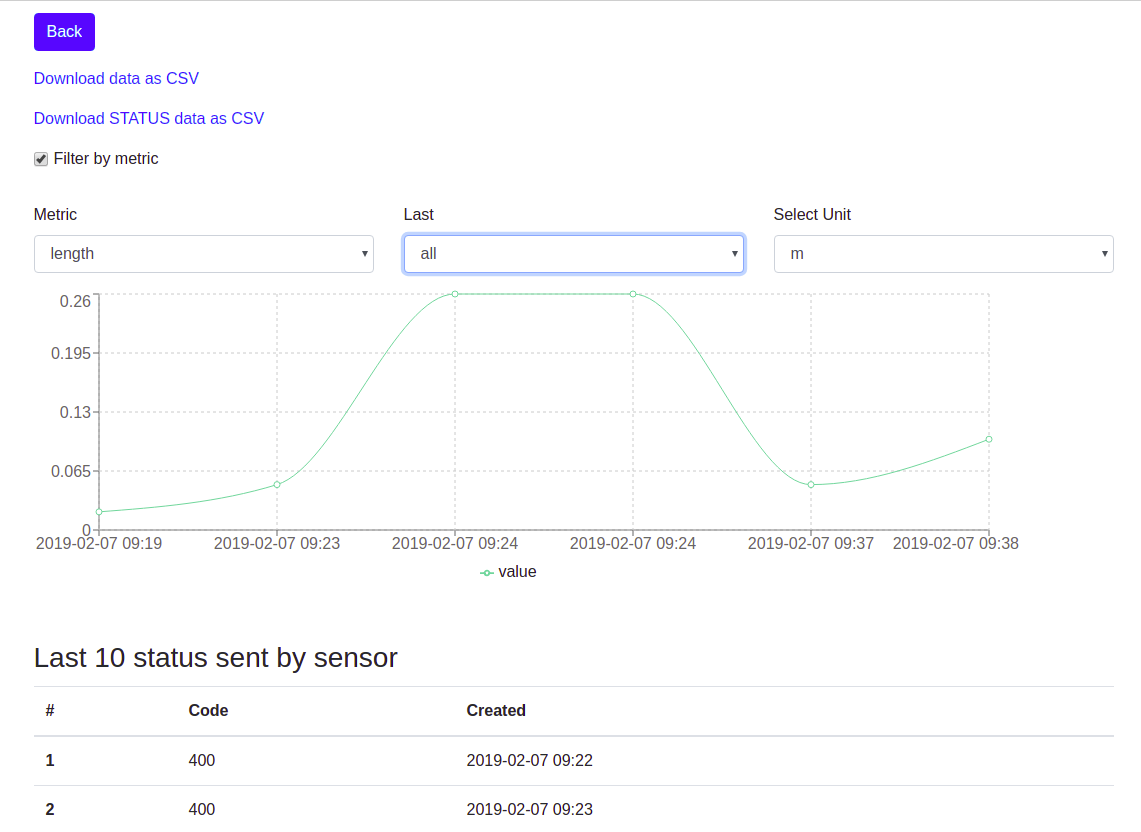
\includegraphics[width=0.95\textwidth]{sensor_detail}
\label{fig:sensor_graph}
\end{figure}

\newpage
\subsection{Přehled senzorů na mapě}
Druhá komponenta (obrázek \ref{fig:overview}) umožňuje zobrazit všechny senzory specifické metriky na mapě (pokud mají vyplněny \textit{lat} a \textit{lng} parametry). Dále je po kliknutí na značku senzoru na mapě zobrazena jeho stručná charakteristika s možností přesměrování na jeho detail. Charakteristika obsahuje minimum, maximum a průměr, ale jen pokud je možný převod na kotevní jednotku. Pro detail senzoru se využívá endpoint \textit{/data/overview/:metricId/:sensorId}
\begin{figure}[h]
\caption{Ukázka mapy s detailem senzoru}
\centering
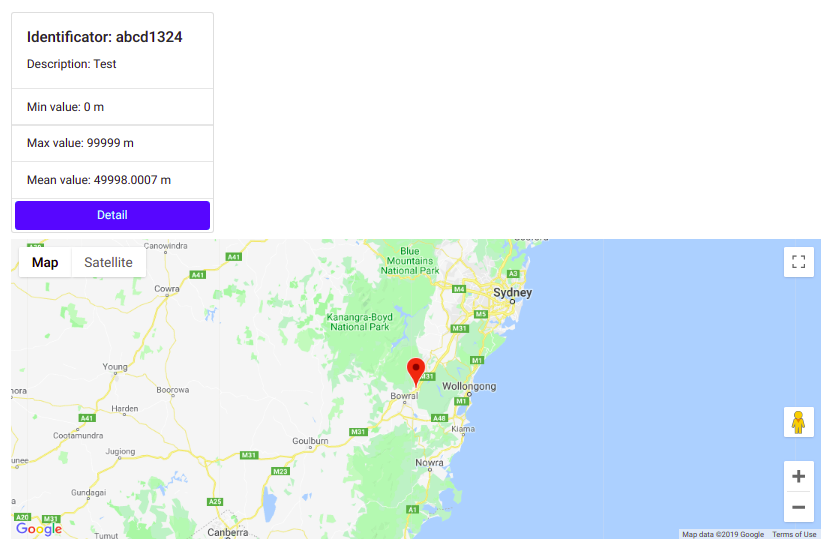
\includegraphics[width=0.95\textwidth]{overview}
\label{fig:overview}
\end{figure}

Tato komponenta je implementována pro dvě platformy poskytující online mapy, a to pro Google Maps a Mapbox.
Použita je ta, která má v konfiguračním souboru \textit{.env} vyplněn API klíč.


\chapter{Testování}\label{impltest}
Testování je stejně jako řešení rozděleno na dvě části, testování frontendu a backendu. Jelikož se většina logiky provádí na backendu, tak mu byla věnována větší pozornost.
	
	Backend aplikace je pokryta unit testy, které například ověřují funkčnost mapovací logiky. Všechny controllery jsou pokryty integračními testy, kde se ověřuje celková funkčnost aplikace. Dále je ověřena správnost řešení otestováním výkonu pomocí zátěžových testů.
	
	U frontend aplikace se testují React komponenty pomocí snapshot testů.
\section{Testování backend aplikace}
Jak již bylo řečeno, tak backend aplikace je pokryta integračními a unit testy. K tomu jsou v této práci použity knihovny Mocha a Chai.
	
	Mocha je testovací framework, který může být spuštěn v Node.js i v browseru. Mocha poskytuje funkcionalitu umožňující testování synchronního i asynchronního kódu. Spolu s Mocha je ale potřeba také použít knihovnu pro porovnání výsledků (assertion library). K tomu je použita knihovna Chai.
	
\subsection{Integrační testy}
Integrační testy pokrývají na backendu všechny controllery se všemi používanými akcemi. Jako příklad implementace je použita nejpoužívanější akce \textit{Login}.
	
	Nejprve je nutné definovat takzvaný test suit, který poté bude obsahovat jednotlivé testy (test cases). K vytvoření test suit se v Chai používá metoda \textit{describe} a k vytvoření test case metoda \textit{it}. To vše jde do sebe vnořovat jako callback funkce. Každý test case obdrží v callback funkci metodu \textit{done}, která je zavolána na konci každého testu.
\newpage
\begin{lstlisting}
  describe('AuthController tests', () => {
    describe('test login process', () => {
      it('it should login and receive token', (done) => {})  
      })  
  })  
\end{lstlisting}
Aby všechny testy byly na sobě navzájem nezávislé, tak je potřeba, aby měly stejná počáteční data, i pokud je test v rámci svého procesu modifikuje. K tomu se nejčastěji používají metody \textit{before} a \textit{beforeEach}. Metoda \textit{before} je spuštěna pouze jednou v rámci své scope, zatímco \textit{beforeEach} před každým jednotlivým testem. V metodě \textit{before} je většinou v této aplikaci vytvářen uživatel, který poté využívá všechny endpointy. Ten se totiž ve většině testů pouze využívá, ale nemodifikuje.
\begin{lstlisting}
    before((done) => {
      const userData = { data testovacího uživatele } 
      User.deleteMany({}) // smazání všech uživatelů
        .then(() => {
          return User.create(userData)
        })
        .then(() => {
          done()
        })
        .catch((err) => {
          throw err
        })  
    })    
\end{lstlisting}

Nyní už je v databázi připraven uživatel, pomocí kterého se může otestovat přihlašovací proces. K tomu je využita metoda \textit{getRequest}, která umožňuje odeslat libovolný požadavek. Na ni v případě přihlášení zavoláme metodu \textit{post}, která přijme jako parametr cestu daného endpointu. V poslední metodě \textit{send} zašleme data potřebná k přihlášení. Poté je už pouze nutné definovat metodu \textit{end}, která jako parametr přijímá callback funkci, která bude zavolána po dokončení požadavku. Tato callback funkce přijme atributy \textit{error} a \textit{response}. V případě chyby jsou v atributu \textit{error} zaslány podrobnosti o příslušném neúspěšném požadavku, zatímco v \textit{response} je zaslána odpověď na validní požadavek. Tato odpověď je následně ověřena pomocí Chai na to, zda obsahuje token, který má v případě úspěšného přihlášení přijít. Na samém konci nesmíme zapomenout zavolat metodu \textit{done}.
\newpage
\begin{lstlisting}
  describe('test login process', () => {
      it('it should login and receive token', (done) => {
        getRequest()
          .post('/auth/login')
          .send({ username: 'user1', password: 'test1' })
          .end((err, res) => {
            res.should.have.status(200)
            res.body.should.be.a('Object')
            expect(res.body.token).to.be.a('string')
            done()
          })  
      })  
    })
\end{lstlisting}
Podobným způsobem jsou testovány všechny ostatní controllery. Jelikož je ale u většiny z nich potřeba přihlášení, tak je předchozí logika přenesena do pomocné funkce \textit{loginAs}, která provádí přihlášení před každým testem.
\subsection{Unit testy}
Unit testy využívají Mocha a Chai stejně jako integrační testy. Unit testy pokrývají veškerou logiku jako konvertování jednotek, parsery, atd. Následující ukázka zobrazuje jeden z testů JSON parseru.
\begin{lstlisting}
  it('Test Valid JSON ID parser', function() {
    const body = '{"id": "idval", "key": {"value": "4"}}'
    const result = JsonIdParser(
      sensorIdMappers,
      JSON.parse(body),
    )
    assert.equal(result, 'idvalue')
  })
\end{lstlisting}
\newpage

\section{Testování frontend aplikace}
Frontend aplikace je složena z mnoha React komponent. K jejich otestování jsou použity snapshot testy. Pomocné funkce jsou otestovány pomocí klasických Unit testů.
\subsection{Snapshot testy}
Snapshot testy slouží k testování React komponent. Pro snapshot testování se využívá testovací knihovna Jest a react-test-renderer, který slouží k vykreslení komponenty, aniž by byl potřeba DOM. 

Snapshot testy fungují tak, že při prvním spuštění se vytvoří ve složce \textit{\_\_snapshots\_\_} soubor, který obsahuje vykreslenou React komponentu v HTML. Vývojář ověří, zda je vygenerovaná správně. Pokud poté dojde k její změně, tak je hlídáno, zda je vygenerovaná opět ve stejné podobě. Pokud však provedeme chtěnou změnu, tak musíme daný snapshot přegenerovat. K tomu slouží Jest příkaz \textit{jest updateSnapshot}.

\begin{figure}[h]
\caption{Přihlašovací komponenta}
\centering
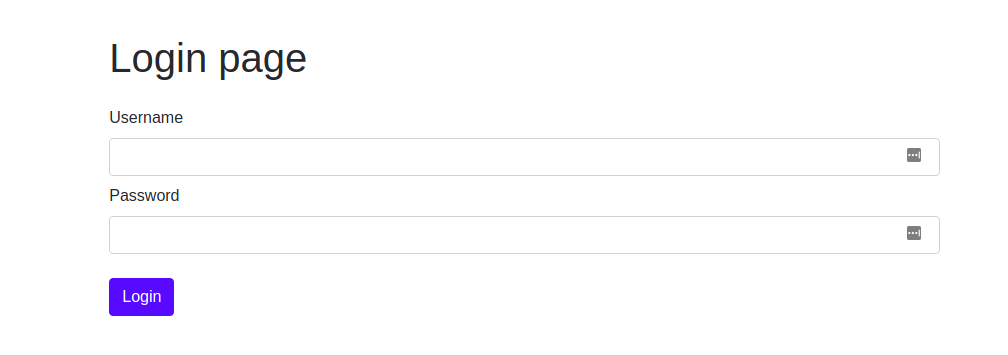
\includegraphics[width=0.95\textwidth]{login}
\label{fig:login}
\end{figure}

Pro ukázku byl vybrán jeden krátký snapshot test přihlašovací stránky. Pro již zhotovenou React komponentu s názvem \textit{Login} (na obrázku \ref{fig:login}), obsahující jednoduchý formulář se vstupem pro přihlašovací jméno a heslo, bude v Jestové defaulní složce \textit{\_\_tests\_\_} vytvořen soubor \textit{login.react.test.js}. Poté je nutné naimportovat React, výše zmíněný renderer a komponentu Login. Poté stačí pouze pomocí metody \textit{create} vykreslit komponentu a porovnat ji s již uloženým snapshotem.
\begin{lstlisting}
  import React from 'react'
  import renderer from 'react-test-renderer'
  import Login from '../src/user/login/Login'
  
  it('renders correctly', () => {
    const tree = renderer.create(<Login />).toJSON()
    expect(tree).toMatchSnapshot()
  })

\end{lstlisting}

\subsection{Unit testy}
Ačkoliv většina logiky se odehrává na API, některé funkce frontendové aplikace vykonávají logiku, kterou je potřeba otestovat.


Jako příklad frontedového unit testu je případ, kdy je potřeba immutabilně modifikovat pole jednotek metriky. K tomu slouží funkce \textit{immutableEditUnit}, která jako parametry přijímá pole jednotek metriky, jednotku, kterou chceme modifikovat a na kterém indexu pole. Následně se musí otestovat nejen požadovaný výstup, ale i jestli nebyl modifikován objekt vstupního pole.

\begin{lstlisting}
  it('immutable edit of unit on specific index', () => {
    const units = [          
      { name: '1', anchor: false, to_anchor: 0.2, },                     
      { name: 'test2', anchor: true, to_anchor: 1, },
    ]
       
    const unitForEdit = 
     { name: 'test2', anchor: false, to_anchor: 0.1, }
       
    const expectedResult = [ 
      { name: '1', anchor: false, to_anchor: 0.2, },                     
      { name: 'test2', anchor: false, to_anchor: 0.1, },
    ]                        
  
    expect(immutableEditUnit(units, unitForEdit, 1))
       .toEqual(expectedResult)
    expect(units[1].anchor).toBe(true)
    expect(units[1].to_anchor).toBe(1)
    expect(units[1].name).toBe('test2')
  })

\end{lstlisting}
\newpage
\section{Test rychlosti}
Jako poslední byl prováděn test rychlosti. Na API bylo sledováno, jak rychle budou požadavky obsluhovány. Na to může mít vliv počet požadavků za sekundu a také velikost databáze. Na frontendu se testoval výkon při větším množství dat, které může mít vliv na vykreslování grafů a plynulost celé aplikace.

\subsection{Frontend}
Testování plynulosti frontendové aplikace bylo zaměřeno hlavně na to, jak budou prezentační funkce jako grafy a export do CSV plynulé při větším množství dat. Při tomto testování bylo odhaleno, že knihovna pro vykreslování grafů Recharts má výkonnostní problémy při větším množství dat (řádově při pěti tisících a výše). To mělo za následek velké množství výpočetních operací. Z toho důvodu byly od určitého počtu dat (tři tisíce) vypnuty všechny animace a různé designové funkce knihovny. To vedlo k mnohem větší plynulosti vykreslování. Export do CSV a další funkce nebyly velkým počtem dat zásadně ovlivněny.
\subsection{Backend}
U dat přicházejících ze senzorů lze očekávat jejich velký nárůst. Z toho důvodu bylo otestováno, jak bude API pracovat, až data budou mít větší množství položek. Přesněji bylo zkoumáno, jak dlouho bude API trvat zpracovat požadavek. Data se totiž nenačtou pouze z databáze a následně neodešlou, ale může na ně být aplikována celá řada funkcí a filtrů. Mezi ně patří:
\begin{enumerate}
\item Očištění samotných dat od databázového identifikátoru a dalších pro frontend aplikaci nepotřebných údajů.
\item Převedení dat na stejnou jednotku (potřebné u vykreslení grafu).
\item Vyfiltrování dat za určitý časový horizont.
\item Stručná charakteristika dat (minimum, maximum a průměr).
\end{enumerate}

Byla zkoumána doba zpracování požadavku API, a to ve výpočetně nejnáročnějším případě. To je, když jsou aplikovány všechny výše zmíněné filtry a funkce. Měření probíhalo na lokálním prostředí.

Schopnost backendu shromažďovat data byla zároveň otestována pomocí senzoru, který poskytl vedoucí práce.
\newpage
\subsection{Test detailu senzoru}

Na detailu senzoru (obrázek \ref{fig:sensor_graph}) se provedla měření s počtem až do sto tisíc položek dat stejné metriky, stejného senzoru a byl zaznamenáván čas. Měření byla u každého množství (100, 1000, 10 000 a 100 000 položek) prováděna desetkrát bez jakékoliv cache a následně zprůměrována. Jako první byl testován endpoint pro získání všech dat za časový horizont jednoho roku převedených na centimetry \textit{/data/sensorId/metricId?convertUnit=cm\&lastDate=years}.

\begin{figure}[h]
\begin{tikzpicture}[scale=\textwidth/11.5cm,samples=200]
	\begin{loglogaxis}[
		xlabel=Počet zpracovávaných dat,
		ylabel=Doba zpracování (ms)]
	\addplot[color=red,mark=x] coordinates {
(100,64 )(1000,125 )(10000,8050 )(100000,80880)
	};
	\end{loglogaxis}
\end{tikzpicture}
\end{figure}

Z výše uvedeného grafu naměřených dat je vidět zhruba lineární nárůst, což je oproti čtení těchto dat z databáze podstatné zhoršení. Jeden z důvodu je, že všechny filtry a funkce se aplikují na sobě nezávisle, a tak se provádí mnoho iterací nad těmito daty. To bylo navrhnuto, aby se funkce mohly aplikovat v libovolném pořadí a počtu. 

Frontend aplikace si však s tímto problémem poradila, jelikož všechna data se načítají asynchronně a uživatel si počká pouze na načtení dílčích částí. V budoucnu je ale rozhodně prostor pro lepší optimalizaci. Dále je nutno podotknout, že dotaz na data senzoru překračující počet několika tisíc položek není pravděpodobný.
\newpage
\subsection{Test mapy}
Druhý test byl proveden u endpointů vracejících všechny senzory a základní statistiky jejich dat (průměr, maximum, minimum), které jsou využity například u mapy (obrázek \ref{fig:overview}). Už při začátku testu bylo odhaleno, že řešení je absolutně nevyhovující. Začala se zpracovávat data všech senzorů, i když nebyla uživatelem označena pro zobrazení detailu. Při deseti senzorech o 1000 položek dat (každý) trvalo načtení přibližně 30 sekund. Dále se v testu tedy nepokračovalo a přepracoval se návrh celého procesu. 


Ve druhé verzi byl pozměněn kompletně proces získání senzorů a dat. Nejprve si frontend aplikace požádá o všechny požadované senzory. Poté, co uživatel označí senzor na mapě pro detail, tak se asynchronně odešle požadavek o data vybraného senzoru. Toto řešení se ukázalo jako ideální a testovatelné. Dále se tedy podobně jako u testu detailu provedl test rychlosti na vzorcích 100, 1000, 10 000 a 100 000 položek. Provolávaný endpoint je \textit{/data/overview/metricId/sensorId}.

\begin{figure}[h]
\begin{tikzpicture}[scale=\textwidth/11.5cm,samples=200]
	\begin{loglogaxis}[
		xlabel=Počet zpracovávaných dat,
		ylabel=Doba zpracování (ms)]
	\addplot[color=red,mark=x] coordinates {
(100,40 )(1000,80 )(10000,280 )(100000,2185)
	};
	\end{loglogaxis}
\end{tikzpicture}
\end{figure}

Díky menšímu počtu možných filtrů dosahuje zkoumaný endpoint lepších výsledků než ten z předešlého testu a spolu s novým řešením celého procesu je výsledek uspokojivý.

\begin{conclusion}

Byly vytvořeny dvě aplikace umožňující správu a konfiguraci IoT projektů. První z nich je navržena v Node.js a je schopna shromažďovat příchozí data ve formátech JSON, text a v binárním formátu, který je reprezentován hexadecimálně. Tato příchozí data jsou ukládána pomocí MongoDB databáze. Aplikace umožňuje vytvářet a modifikovat informace o skupinách, uživatelích, senzorech, metrikách a mapperech, které umožňují příchozí data zpracovávat. Dále je umožněno data zobrazovat jen povolaným osobám v rámci jejich ranku a skupin. Tato aplikace je obsluhována jako RESTful API. Druhá aplikace toto RESTful API využívá a umožňuje jeho snadné používání pomocí interaktivního UI implementovaného v Next.js a React. Zároveň prezentuje výsledná data pomocí grafů a mapy. Obě aplikace jsou otestovány tak, jak je definováno v zadání. Zároveň proběhl test použitím skutečného senzoru, který poskytl vedoucí práce.


Tyto aplikace mohou být dále rozšiřovány o další funkcionality. V budoucnu je například možnost umožnit zpracovávat další formáty jako XML a další reprezentace binárních dat, či optimalizovat výkon zpracovávání dat. Dále je možné rozšířit aplikaci o možnost, existence více správců, kteří mohou spravovat své senzory, aniž by do nich ostatní správci mohli zasahovat, či zpřístupnit tuto možnost dokonce uživatelům.
\end{conclusion}
\bibliographystyle{csn690}
\bibliography{mybibliographyfile}
\nocite{*}
\appendix
\chapter{Seznam použitých zkratek}
% \printglossaries
\begin{description}
	\item[API] Application Programming Interface
	\item[CSS] Cascading Style Sheets
	\item[CSV] Comma-separated values
	\item[JSON] JavaScript Object Notation
	\item[SASS] Syntactically Awesome Style Sheets
	\item[REST] Representational State Transfer
	\item[HTTP] Hypertext Transfer Protocol
	\item[URI] Uniform Resource Identifier
	\item[URL] Uniform Resource Locator
	\item[HTML] Hypertext Markup Language 
	\item[IoT] Internet of Things
	\item[CI] Continuous integration
	\item[BSON] Binary JavaScript Object Notation 
	\item[UI] User interface
	\item[DOM] Document Object Model
	\item[JWT] JSON web token
	\item[URL] Uniform Resource Locator
	\item[MVC] Model-view-controller
\end{description}

\chapter{Obsah přiloženého CD}

%change appropriately

\begin{figure}
	\dirtree{%
		.1 readme.txt\DTcomment{Popis obsahu CD}.
		.1 src\DTcomment{Složka se zdrojovými kódy}.
		.2 README\DTcomment{Manuál k instalaci a obsluze aplikací}.
		.2 frontend\DTcomment{Zdrojové kódy frontend aplikace}.
		.2 backend\DTcomment{Zdrojové kódy backend aplikace}.	
		.2 thesis\DTcomment{Složka s \LaTeX{} zdrojovými kódy práce}.
		.1 text\DTcomment{Text diplomové práce}.
		.2 thesis.pdf\DTcomment{Text diplomové práce v PDF formátu}.
	}
\end{figure}
\end{document}
